\documentclass[12pt]{report}
\usepackage[margin=1in, a4paper]{geometry}

\title{Ekalavya Summer Internship 2019}
\author{Ekalavya Interns}

\ifx\pdftexversion\undefined
\usepackage[dvips]{graphicx}
\else

\usepackage[pdftex]{graphicx}
\DeclareGraphicsRule{*}{mps}{*}{}
\fi
\usepackage{url}
\usepackage{chapterbib}
\usepackage{hyperref}
\usepackage{lscape}
\usepackage{longtable}
\usepackage{float}
\usepackage{url}
\usepackage{multicol}
\usepackage{color}
\usepackage{textcomp}

\usepackage{fancyhdr}
\pagestyle{fancy}
\lhead{\leftmark}
\rhead{Project: P3}
\lfoot{Fundamental Research Group, IIT Bombay}
\cfoot{ }
\rfoot{\thepage}

\renewcommand{\bibname}{References}
\newcommand\tab[1][1cm]{\hspace*{#1}}

\setcounter{secnumdepth}{4}
\setcounter{tocdepth}{4}

\begin{document}
	%***********************
	%Title page
	\begin{titlepage}
		\begin{center}
			\begin{figure}[h]
				\centering
				
\includegraphics[width=8cm]{./iitb-black.pdf}
			\end{figure}
			
			INDIAN INSTITUTE OF TECHNOLOGY, BOMBAY\\
			EKLAVYA SUMMER INTERNSHIP 2019\\
			(FUNDAMENTAL RESEARCH GROUP) 
			\noindent\rule{15cm}{0.4pt}\\
			\textbf{\huge \\Configurable and Scalable IITBombayX MOOC platform on commodity servers}\\
			\textbf{}\\
			\noindent\rule{15cm}{0.4pt}
			\newline
			\\Under the guidance of: \textbf{Prof. S. Sudarshan}
			\begin{multicols}{2}
				\textbf{\\ \large
					\textbf{Team:} \\
					\textbf{Amit Kumar Tiwari}\\
					\textbf{Harshit Mogalapalli}\\
					\textbf{Mridul Mahajan}\\
					\textbf{Ritik Kumar}\\
					\textbf{Soumyakant Mohakul}\\
				}
				\columnbreak
				\textbf{\\ \large
					\textbf{Mentors:}\\
					\textbf{Mr. Nagesh Karmali}
				}
			\end{multicols}
			
		\end{center}
	\end{titlepage}
	%*****************************
	
	%certificate area
	%*************************
	\pagebreak
	\newpage
	\thispagestyle{empty}
	
	\begin{center}
		\huge{Summer Internship 2019 Project}\\[0.5cm]
		Approval Certificate\\[1.0cm]
		\huge{Department of Computer Science and Engineering}\\[0.5cm]
		\normalsize
		\textsc{Indian Institute of Technology Bombay}\\[2.0cm]
		
		\emph{\LARGE Certificate}\\[2.5cm]
	\end{center}
	\normalsize The project entitled Configurable and Scalable IITBombayX MOOC platform on commodity servers submitted by Mr. Amit Kumar Tiwari, Mr. Harshit Mogalapalli, Mr. Mridul Mahajan, Mr. Ritik Kumar and Mr. Soumyakant Mohakul is approved for Summer Internship 2019 programme from 19th May 2019 to 9th July 2019, at Department of Computer Science
	and Engineering, IIT Bombay.\\[1.0cm]
	
	\begin{multicols}{2}
		\noindent\rule{5cm}{0.4pt}\\
		\textbf{\\DR. S. SUDARSHAN} \\
		Dept. of CSE, IITB \\
		Principle Investigator \\
		\columnbreak
		
		\noindent\rule{5cm}{0.4pt}\\
		\textbf{\\MR. NAGESH KARMALI} \\
		Dept. of CSE, IITB \\
		Project-In-Charge \\
		\textbf{\\\\}
	\end{multicols}
	
	\begin{flushleft}
		Date:\today \\
		Place:
	\end{flushleft}
	\pagebreak
	%*************************
	
	\setcounter{page}{1}
	\pagenumbering{roman}
	
	\listoffigures
	
	\pagebreak
	
	\listoftables
	
	\pagebreak
	
	\tableofcontents
	
	\pagebreak
	
	\setcounter{page}{1}
	\pagenumbering{arabic}
\section{Acknowledgement}
We have spent a lot of effort on this project. However, it would not have been possible without the kind support of various individuals and organizations, we would like to extend our sincere thanks to all of them.
\\
\\
We would like to express our sincere thanks and regards to Prof S. Sudarshan and Indian Institute of Technology, Bombay for providing us this unparalleled opportunity to work on this esteemed project. We would also like to extend our sincere thanks to Mr. Nagesh Karmali for supervising our project. Our sincere thanks to Mrs. K. Revathi, Mr. Gaurav Ojha \& Mr. Gaurav Patil without whom the project would not be this refined and successful.
\\ 
\\

\pagebreak

%***************************************
%Declaration Page
%***************************************
\section{Declaration}
\textbf{\\}
I declare that this written submission represents my ideas in my own words and where others’ ideas or words have been included, I have adequately cited and referenced the original sources. I also declare that I have adhered to all principles of academic honesty and integrity and have not misrepresented or fabricated or falsified any idea/data/fact/source in my submission. I understand that any violation of the above will be cause for disciplinary action by the institute.
\textbf{\\\\\\\\}
\begin{multicols}{2}
	\noindent\rule{5cm}{0.4pt}\\
	\textbf{\\AMIT KUMAR TIWARI} \\
	MMMUT GORAKHPUR\\
	\textbf{\\\\\\}
	\noindent\rule{5cm}{0.4pt}\\
	\textbf{\\HARSHIT MOGALAPALLI} \\
	NIT TIRUCHIRAPPALLI\\
	\textbf{\\\\\\}
	\noindent\rule{5cm}{0.4pt}\\
	\textbf{\\MRIDUL MAHAJAN} \\
	IIIT ALLAHABAD\\
	\textbf{\\\\\\}
	\columnbreak
	
	\noindent\rule{5cm}{0.4pt}\\
	\textbf{\\RITIK KUMAR} \\
	NIT AGARTALA\\
	\textbf{\\\\\\}
	\noindent\rule{5cm}{0.4pt}\\
	\textbf{\\SOUMYAKANT MOHAKUL} \\
	IIT BHILAI\\
	\textbf{\\\\}
\end{multicols}
\pagebreak
\chapter{Introduction}
\section{Aim of the project}

The aim of this project is to deploy an instance of Open edX MOOC platform on a multi-node cluster using Kubernetes as the container orchestrator and Docker as the container runtime environment. \\

\textbf{Technologies used:}
\begin{itemize}
	\item Docker
	\item Kubernetes
	\item Ansible
	\item Shell scripting
	\item Git
	\item Cluster management and configuration
\end{itemize}
%Paste appropriate content from here. 

%The following is an example of inserting an image which is shown in Figure ~\ref{fig:Image1} 

%\begin{figure}[hb]
%\centering
%
\includegraphics[width=12cm]{./Image1.jpg}
%\caption{Name of the Figure\label{fig:Image1}}
%\end{figure}

\section{Open edX}
Open edX is an open source online MOOC platform to create and deliver online courses. It provides both web and mobile platforms to clone the basic template of e-learning platform. In this project, we have worked on the web platform.

\subsection{Releases}
Open edX has multiple releases. Some of the most recent ones are:
\begin{itemize}
	\item Ironwood
	\item Hawthorn
	\item Ginkgo
\end{itemize}
We have used the Ironwood.1 release in this project.

\subsection{Installation}
Open edX can be installed in two ways:
\begin{itemize}
	\item Native installation
	\item Docker-based installation
\end{itemize}
\subsubsection{Native installation}
\textbf{i) Prerequisites}
\begin{itemize}
	\item Ubuntu 16.04 amd64
\end{itemize}
\textbf{ii) Set-up configurations}\\\\
Ubuntu package sources need to be updated:\\\\
\textbf{\$ sudo apt-get update -y\\
	\$ sudo apt-get upgrade -y\\
	\$ sudo reboot\\\\
}
\textbf{iii) Installation procedure}
\begin{enumerate}
	\item Set the OPENEDX\_RELEASE variable to the Git Tag corresponding to the Ironwood release of Open edX:\\\\
	\textbf{export OPENEDX\_RELEASE=open-release/ironwood.1}
	\item Next, create a config.yml file, which states the hostname of the Learning Management System (LMS) and the Content Management System (CMS):\\\\
	\textbf{EDXAPP\_LMS\_BASE: “127.0.0.1”}\\
	\textbf{EDXAPP\_CMS\_BASE: “127.0.0.1:8080”}\\\\
	(works only when the LMS hostname and the CMS hostnames are the same, or the CMS hostname is a subdomain of the LMS hostname).
	\item Now bootstrap the Ansible installation.
	\item Retrieve the ansible-bootstrap.sh bash script from the Github server and execute it:\\\\
	\textbf{wget https://raw.githubusercontent.com/edx/configuration/\\ \$OPENEDX\_RELEASE/util/install/ansible-bootstrap.sh -O - $|$ sudo bash}
	\item Use the generate-password.sh file from the Github server to randomize password:\\\\
	\textbf{wget https://raw.githubusercontent.com/edx/configuration/\\ \$OPENEDX\_RELEASE/util/install/generate-passwords.sh -O - $|$ bash}
	\item Finally, use the native.sh script from the Github server to install Open edX:\\\\
	\textbf{wget https://raw.githubusercontent.com/edx/configuration/\\ \$OPENEDX\_RELEASE/util/install/native.sh -O - $|$ bash}
	
\end{enumerate}
\subsubsection{Docker-based installation}
\label{sec:dockerinstall}
\textbf{i) Installing docker engine, docker machine and docker compose:}
\\ \\
The docker based installation allows the resources of our system to be utilized in an optimal way. Docker is based on the principle of containerization. For Open edX Devstack to work properly, we would need the Docker engine, Docker Machine and Docker Compose tools.\\ \\
For installing the docker engine, the following commands need to be run:
\begin{enumerate}
	\item \$ sudo apt-get update
	\item \$ sudo apt-get install \textbackslash \\
	apt-transport-https \textbackslash \\
	ca-certificates \textbackslash \\
	curl \textbackslash \\
	gnupg-agent \textbackslash \\
	software-properties-common
	\item \$ curl -fsSL https://download.docker.com/linux/ubuntu/gpg | sudo apt-key add -
	\item \$ sudo apt-key fingerprint 0EBFCD88
	\item \$ sudo add-apt-repository \textbackslash \\
	"deb [arch=amd64] https://download.docker.com/linux/ubuntu \textbackslash \\
	\$(lsb\_release -cs) \textbackslash \\
	stable"
	\item \$ sudo apt-get update
	\item \$ sudo apt-get install docker-ce docker-ce-cli containerd.io
	\item \$ apt-cache madison docker-ce
	\item \$ sudo apt-get install docker-ce=$<VERSION\_STRING>$\\docker-ce-cli=$<VERSION\_STRING>$ containerd.io
\end{enumerate}
\textbf{In order to test if Docker has been installed properly, one can run the following \\command:\\}
\$ sudo docker run hello-world\\\\
For installing docker machine, run the following commands:\\ \\
base=https://github.com/docker/machine/releases/download/v0.16.0 \ \&\& \\
curl -L \$base/docker-machine-\$(uname -s)-\$(uname -m)$>$/tmp/docker-machine \ \&\& \\
sudo install /tmp/docker-machine /usr/local/bin/docker-machine\\ \\
For installing docker compose, run the following commands:
\begin{enumerate}
	\item \$ sudo curl -L "https://github.com/docker/compose/releases/download/1.24.0/docker-compose-\$(uname -s)-\$(uname -m)" -o /usr/local/bin/docker-compose
	\item \$ sudo chmod +x /usr/local/bin/docker-compose
\end{enumerate}
For checking if the tools mentioned above have been installed properly, you can use the \ -\ -version flag with the corresponding command to check the installed version.\\\\
\textbf{ii) Installing Ironwood Devstack:} \\ \\
The three most recent versions of the Open edX Devstack are Ginkgo, Hawthorn and Ironwood. \\\\
The following commands perform the Ironwood-release installation of Devstack:
\begin{enumerate}
	\item git clone https://github.com/edx/devstack
	\item cd devstack
	\item git checkout open-release/ironwood.master
	\item export OPENEDX\_RELEASE=ironwood.master
	\item make dev.checkout
	\item make dev.clone
	\item make dev.provision
\end{enumerate}
On successfully running dev.provision, you will have 15 docker-containers running. The list of them can be obtained using the command:  docker ps
\\\\
The list of docker-containers are: \href{https://drive.google.com/open?id=0B168SrnPp4BpZ1RCQ1VncU81VEZYanl2SUNWN2dtRUg1bGRv}{Docker-containers List}
\\\\
The Provision Log for the tasks executed are: \href{https://drive.google.com/open?id=0B168SrnPp4BpclQ3d3gwbDNWLWtrUzduYUt6Vko4S2h6bzBz}{provision.log}\\\\
\textbf{iii) Errors:}
\begin{enumerate}
	\item  ./provision.sh: line 21: /usr/local/bin/docker-compose: Permission denied
	Makefile:59: recipe for target 'dev.provision.run' failed
	make: *** [dev.provision.run] Error 126\\\\
	\textbf{Solution :}\\\\
	\$ sudo -i\\
	\$ curl -L https://github.com/docker/compose/releases/download/1.18.0/docker-compose-`uname -s`-`uname -m` -o /usr/local/bin/docker-compose\\
	\$ chmod 755 /usr/local/bin/docker-compose\\
	\$ exit
	\item TASK [common : Update expired apt keys] **************
	fatal: [127.0.0.1]: FAILED! => {"changed": true, "cmd": "apt-key adv -{}-recv-keys --keyserver keyserver.ubuntu.com 69464050", "delta": "0:02:00.744139", "end": "2019-05-24 07:49:07.605347", "failed": true, "rc": 2, "start": "2019-05-24 07:47:06.861208", "stderr": "gpg: requesting key 69464050 from hkp server keyserver.ubuntu.com\textbackslash ngpg: keyserver timed out\textbackslash ngpg: keyserver receive failed: keyserver error", "stdout": "Executing: /tmp/tmp.NmWIivV5Jo/gpg.1.sh -{}-recv-keys\textbackslash n-{}-keyserver\textbackslash nkeyserver.ubuntu.com\textbackslash n69464050", "stdout\_lines": ["Executing: /tmp/tmp.NmWIivV5Jo/gpg.1.sh -{}-recv-keys", "-{}-keyserver", "keyserver.ubuntu.com", "69464050"], "warnings": []}
	to retry, use: -{}-limit @/edx/app/edx\_ansible/edx\_ansible/playbooks/demo.retry\\\\
	\textbf{Solution :}\\\\
	This error occurs due to the fetching to apt-keys from an expired link.\\
	To resolve follow the following steps :
	\begin{enumerate}
		\item sudo exec -it edx.devstack.lms bash
		\item cd app/edx\_ansible/edx\_ansible/playbooks/roles/common\_vars/defaults/
		\item vi main.yml
		\item On entering the main.yml file in vim editor change the link for the keyword 
		COMMON\_EDX\_PPA\_KEY from keyserver.ubuntu.com to  hkp://keyserver.ubuntu.com:80
		\item exit
	\end{enumerate}
\end{enumerate}

\chapter{Docker}
\section{About Docker}
Docker is an open-source software tool designed to automate and ease the process of creating, packaging, and deploying applications using an environment called a container. Using application running as a docker conatiner removes the system dependency of the application. No changes has to be made in applications to run them in different environments or machines. Docker based application provides liberty to the developer,tester and deployer to run the same application which any changes specific to their environment. \cite{Docker}
\section{Terms related to Docker}
\subsection{Containerization}
Containerization is a lightweight alternative to full machine virtualization that involves encapsulating an application within a container with its own operating environment. Essentially, containers share the kernel space with the host OS, but have a separate user space. This makes them lightweight.
\subsection{Docker Image}
A \textit{Docker Image} is the basic unit for deploying a Docker container. A Docker image is essentially a static snapshot of a container, incorporating all of the objects needed to run a container.\\\\
\textbf{TLS handshake timeout error in pulling Docker image :}\\\\
In case there is a TLS handshake timeout error while pulling a Docker image from an online repository, try running the command again and again and eventually the image will be pulled:
\begin{figure}[h!]
	\begin{center}
		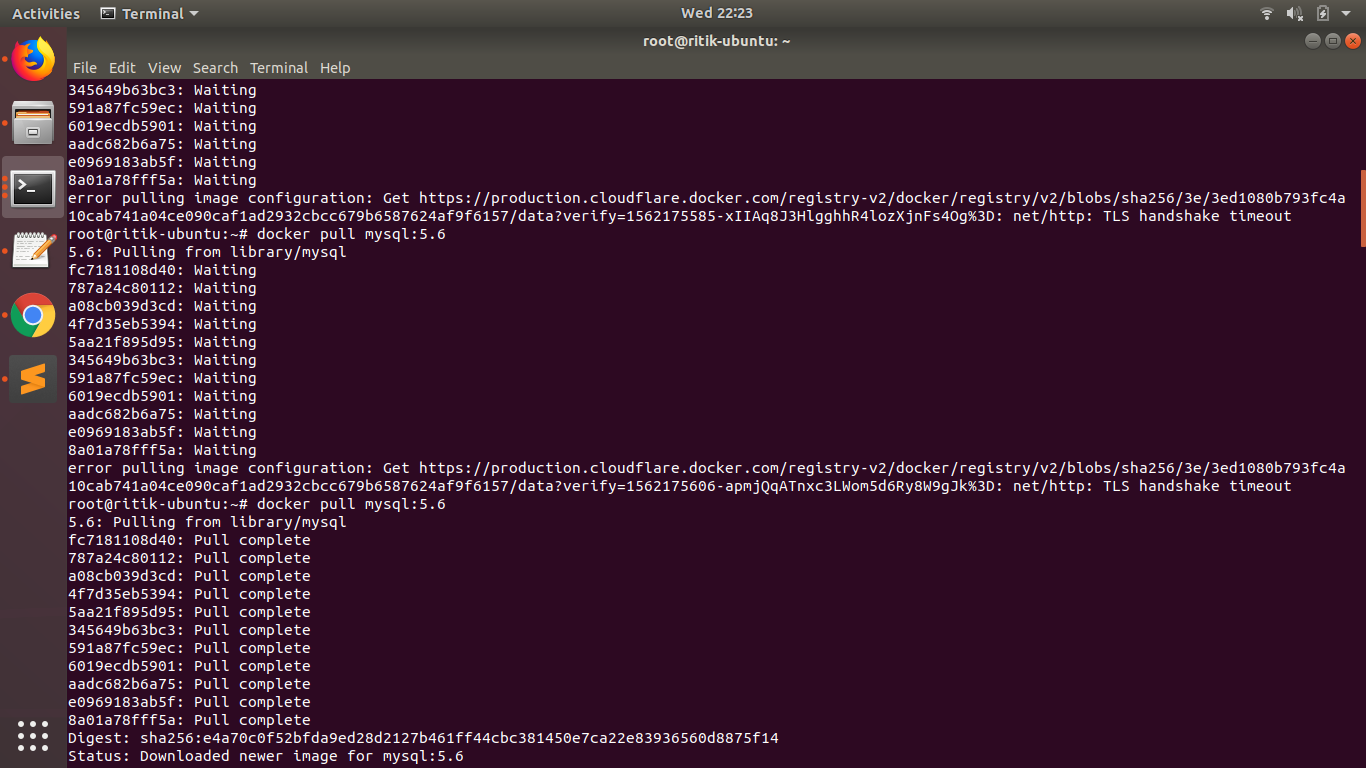
\includegraphics[totalheight=0.4\textheight]{TLS}
		\caption{TLS handshake timeout error}
	\end{center}
\end{figure} 
\subsection{Docker Container}
A \textit{Docker Container} encapsulates a Docker image and when live and running, is considered a container. Each container runs in an isolated environment on the host machine.
\subsection{Docker Registry}
The \textit{Docker Registry} is a stateless, highly scalable server-side application that stores and distributes Docker images. This registry holds Docker images, along with their versions and, it can provide both public and private storage location. There is a public Docker registry called \href{https://hub.docker.com/}{Docker Hub}\cite{Dockerhub} which provides a free-to-use, hosted Registry, plus additional features like organization accounts, automated builds, and more. Users interact with a registry by using Docker push or pull commands.
\subsection{Docker Engine}
The \textit{Docker Engine} is a layer which exists between containers and the Linux kernel and runs the containers. It is also known as the Docker daemon. Any Docker container can run on any server that has the Docker-daemon enabled, regardless of the underlying operating system.
\subsection{Docker Compose}
\textit{Docker Compose} is a tool that defines, manages and controls multi-container Docker applications. With Compose, a single configuration file is used to set up all of your application’s services. Then, using a single command, you can create and start all the services from that file.
\subsection{Dockerfiles}
Dockerfiles are merely YAML configuration files that contains all of the configuration information and commands needed to assemble a container image. With a Dockerfile, the Docker daemon can automatically build the container image.
\section{Docker-Machine}
Docker Machine can be used to :
\begin{itemize}
	\item Manage and provision multiple remote Docker hosts.
	\item Provision Swarm clusters.
\end{itemize}
Docker Machine is a tool that lets you install Docker Engine on virtual hosts, and manage hosts with docker-machine commands. Using docker-machine command you can start, inspect, stop and restart a managed host, upgrade the Docker client and daemon, and configure a Docker client to talk to your host.
\subsection{Install Docker Machine:}
\begin{itemize}
	\item For Linux systems, execute the following command:\\\\
	\textbf{\$ base=https://githubcom/docker/machine/releases/download/v0.16 \&\& curl -L \$base/docker-machine-\$(uname -s)-\$(uname -m) $>$/usr/local/bin/docker-machine \&\& chmod +x /usr/local/bin/docker-machine}
	\item Check the installation by displaying the Machine version:\\\\
	\textbf{\$ docker-machine version}
\end{itemize}
\subsection{Use Docker Machine to run Docker Containers:}
\begin{itemize}
	\item Create a new docker virtual machine.
	\item Switch your environment to your new VM.
	\item Use the docker client to create, load and manage containers.
\end{itemize}
\subsection{Create a Machine}
\textbf{\$ docker-machine create --driver virtualbox default}
\subsection{Connect your shell to the new machine}
\textbf{\$eval “\$(docker-machine env default)”}
\subsection{Run containers and experiment with machine commands}
\begin{itemize}
	\item Use \textbf{docker-run} to download and run images
	\item Run \textbf{docker-machine ip default} to get the host IP address.
	\item Run \textbf{docker-machine stop default} to stop the host default.
	\item Run \textbf{docker-machine start default} to start the host default.
	\item Run \textbf{docker-machine env -u} to see which Docker variables we need to unset to switch to the current shell.
\end{itemize}
\section{Docker Swarm}
Docker swarm is used to create a cluster of nodes. Multi-container, multi-machine applications are made possible by joining multiple machines into a “Dockerized” cluster called a swarm. Docker swarm is a group of machines running docker and are connected to each other by means of an overlay network. There can be one or multiple nodes that can manage the swarm, these nodes are called manager nodes. The rest of the nodes only provide capacity to run the containers and are called worker nodes. 
\subsection{Types of networks in docker}
\begin{itemize}
	\item \textbf{Bridge Network : }This is the type of network that allows the docker containers to communicate within a single host system. This type of network is not feasible to communicate between multiple host systems.\\\\
	A bridge network can be created by :\\
	\textbf{\$ docker network create -{}-driver bridge mynetwork}\\\\
	User-defined bridge networks are best when you need multiple containers to communicate on the same Docker host.
	\item \textbf{Overlay Network : }An overlay network is used for multi host network communication. It connects multiple docker daemons together and enables swarm services to communicate with each other. A docker swarm must always be connected via an overlay network.\\\\
	An overlay network can be created by :\\
	\textbf{\$ docker network create --driver overlay mynetwork}\\\\
	Overlay networks are best when you need containers running on different Docker hosts to communicate, or when multiple applications work together using swarm services.
	\item \textbf{Macvlan Network : }Macvlan networks allow you to assign a MAC address to a container, making it appear as a physical device on your network. The Docker daemon routes traffic to containers by their MAC addresses.\\\\
	A Macvlan Network can be created by :\\
	\textbf{\$ docker network create -d macvlan \textbackslash \\
		-{}-subnet=192.168.40.0/24 \textbackslash \\
		-{}-gateway=192.168.40.1 \textbackslash \\
		-o parent=eth0 my-macvlan-net\\\\
	}
	Macvlan networks are best when you are migrating from a VM setup or need your containers to look like physical hosts on your network, each with a unique MAC address.
	\item \textbf{Host Network : }For standalone containers, remove network isolation between the container and the Docker host, and use the host’s networking directly.\\\\
	We can use the host’s system network to at a particular port to allow the container to share data. Host networks are best when the network stack should not be isolated from the Docker host, but you want other aspects of the container to be isolated.
\end{itemize}
\subsection{Initialising a Swarm Node as Manager}
In order to initialize a swarm node a manager we need to find the IP address of the node using the command \textbf{ifconfig}. Then run the command:\\\\
\textbf{\$ docker swarm init --advertise-addr IP\_OF\_THE\_MANAGER}\\\\
The join token for another node as a manager can be found by :\\\\
\textbf{\$ docker swarm join-token manager\\\\}
The join token of another node as a worker can be found by :\\\\
\textbf{\$ docker swarm join-token worker}
\subsection{Docker Stack}
For multiple services that are dependent on each other to communicate with each other on a swarm network, we may use the Docker Stack command. Docker stack deployment is used to deploy a list of interdependent services on a swarm network.\\\\
To deploy a stack we create a docker-compose file with an additional feature in each service as deploy.\\\\
\textbf{\$ docker stack deploy -c docker-compose.yml myapp}\\\\
The -c flag is used to execute the docker compose file and create multiple interdependent services which can communicate with each other via the swarm network.\\\\
\chapter{Ansible}
Installing docker, kubernetes, and all the other components in each node in a multi-node cluster, which contains many nodes, can be a tedious task. To overcome this issue, Ansible can be used for configuration management. Furthermore, Ansible can be used to configure the nodes too. By default Ansible uses a native openSSH connection and runs commands simultaneously on multiple nodes. We have created Ansible Playbooks for all the needed configurations.
\section{Installing openssh}
\$ sudo apt-get install openssh-server\\
\$ sudo apt-get install openssh-client
\section{Generating key at server and copying in client}
\$ ssh-keygen (generate ssh-key)\\
Copy this key to all nodes to avoid the need to enter a password each time while connecting to the node.\\
To copy ssh-key type command:\\
\$ ssh-copy-id $username@IP\_address$\\\\
\textbf{E.g.:} ssh-copy-id node1@10.130.154.3
\section{Ansible setup}
\subsection{Adding repository}
\$ sudo apt-add-repository ppa:ansible/ansible\\
\$ sudo apt-get update
\subsection{Installing ansible}
\$ sudo apt-get install ansible
\subsection{Checking version}
\$ ansible  --version
\subsection{Ansible directories}
\$ ls -lha /etc/ansible/
\subsection{Making a copy a directory for our use}
\$ cp -R /etc/ansible/ myplatform\\\\
Uncomment the 'inventory = hosts' line in the file ansible.cfg\\\\
\$ vi ansible.cfg \\\\
remove all and write all nodes in new line\\\\
\$ vi hosts \\\\
Add the IP addresses of all the nodes in your cluster on which you want to run the playbooks. Password for each node in the cluster should be the same in order to run commands requiring sudo priviledges.\\\\
\textbf{NOTE :} In case you are running an Ansible playbook for a cluster of nodes having different passwords, you can use multiple vaults. For more details visit \href{https://docs.ansible.com/ansible/latest/user_guide/playbooks_vault.html#multiple-vault-passwords}{https://docs.ansible.com/\\ansible/latest/user\_guide/playbooks\_vault.html\#multiple-vault-passwords}\cite{Ansiblevaults}\\\\ 
\textbf{You can check if all the nodes working by running:}\\
\$ ansible -m ping all
\section{Some useful commands for ansible}
\subsection{To see the hostnames of all nodes}
\$ ansible -m shell -a 'hostname' all
\subsection{To see the volumes used by all nodes}
\$ ansible -m shell -a 'df -h' all
\subsection{To run an ansible-playbook}
\$ ansible-playbook  -K playbook-docker.yml
\chapter{Kubernetes}
\section{What is Kubernetes}
Kubernetes is a container-orchestration tool developed by Google in 2015 and later donated to CNCF (Cloud Native Computing Foundation). Kubernetes provides a smart way for orchestration in setting a multi-node cluster. Kubernetes comes with a lot of functionalities such as load balancing, pod scaling, process scheduling and process management.\cite{Kubernetes}
\section{Main Features Of Kubernetes}
\begin{itemize}
	\item \href{https://kubernetes.io/docs/concepts/services-networking/service/}{Service discovery and load balancing}\cite{Kservice}
	\item \href{https://kubernetes.io/docs/concepts/storage/persistent-volumes/}{Storage orchestration}\cite{Kstorch}
	\item \href{https://kubernetes.io/docs/concepts/configuration/manage-compute-resources-container/}{Automatic bin packing}\cite{Kmanage}
	\item \href{https://kubernetes.io/docs/concepts/workloads/controllers/replicationcontroller/#how-a-replicationcontroller-works}{Self-healing}\cite{Kcontrol}
	\item \href{https://kubernetes.io/docs/concepts/workloads/controllers/deployment/}{Automated rollouts and rollbacks}\cite{Krollout}
	\item \href{https://kubernetes.io/docs/concepts/configuration/secret/}{Secret and configuration management}\cite{Kscmanage}
	\item \href{https://kubernetes.io/docs/concepts/workloads/controllers/jobs-run-to-completion/}{Batch execution}\cite{Kbe}
	\item \href{https://kubernetes.io/docs/tasks/run-application/horizontal-pod-autoscale/}{Horizontal scaling}\cite{Khs}
\end{itemize}
\section{Terminologies in Kubernetes}
\subsection{Pod}
The most fundamental unit in a kubernetes cluster is a pod. A pod is a collection of container and volumes. Each pod is assigned an IP address.\\
\begin{figure}[h!]
	\begin{center}
		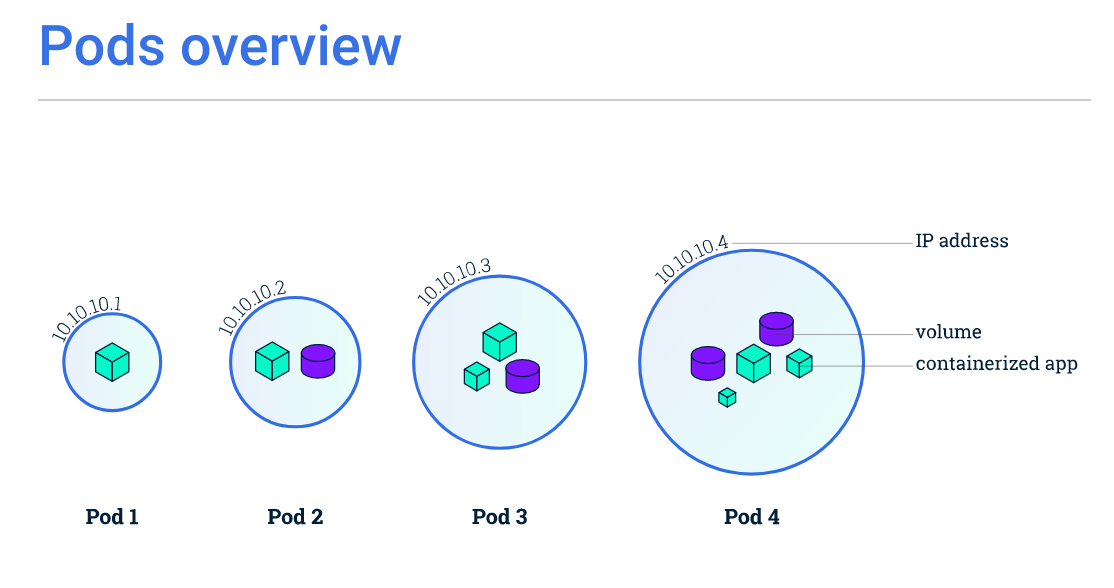
\includegraphics[width=\textwidth, trim= 0 0 0 7cm, clip=true]{pods}
		\caption{Kubernetes pods \cite{Pods}}
	\end{center}
\end{figure}
\subsection{Deployment}
A deployment can be seen as a stateless state of the pod. A deployment is used to provide pod definition and rolling updates to the pod. A deployment contains information such as number of replicas, image, volume mount, hostname and restart policy.\\
\begin{figure}[h!]
	\begin{center}
		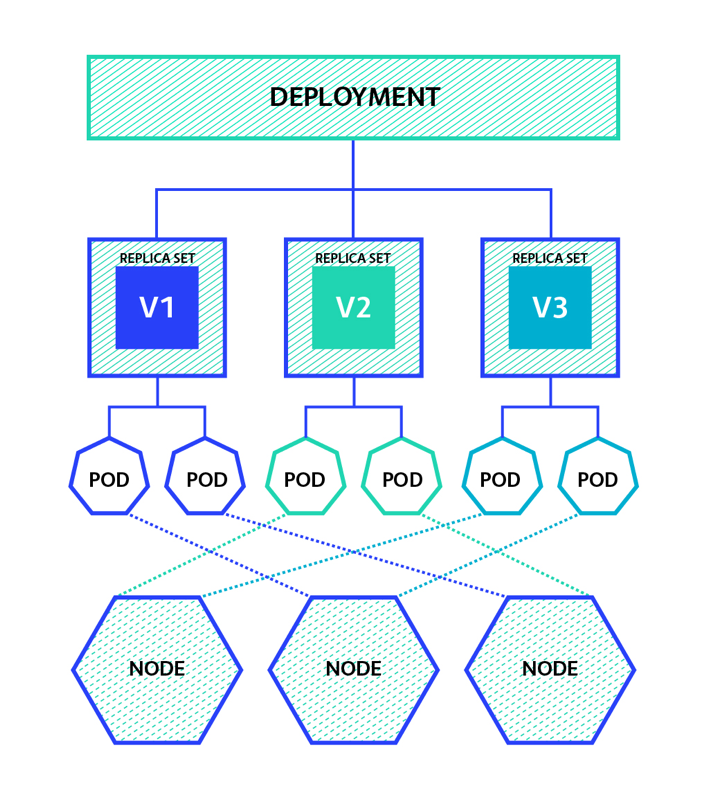
\includegraphics[totalheight=0.45\textheight]{deploy}
		\caption{Kubernetes deployment \cite{Deployments}}
	\end{center}
\end{figure}
\subsection{Service}
A service exposes a deployment as a network service. A deployment is stateless whereas a service can be considered as a stateful definition. The three types of services in kubernetes are: ClusterIP, NodePort and LoadBalancer.\\
\begin{figure}[h!]
	\begin{center}
		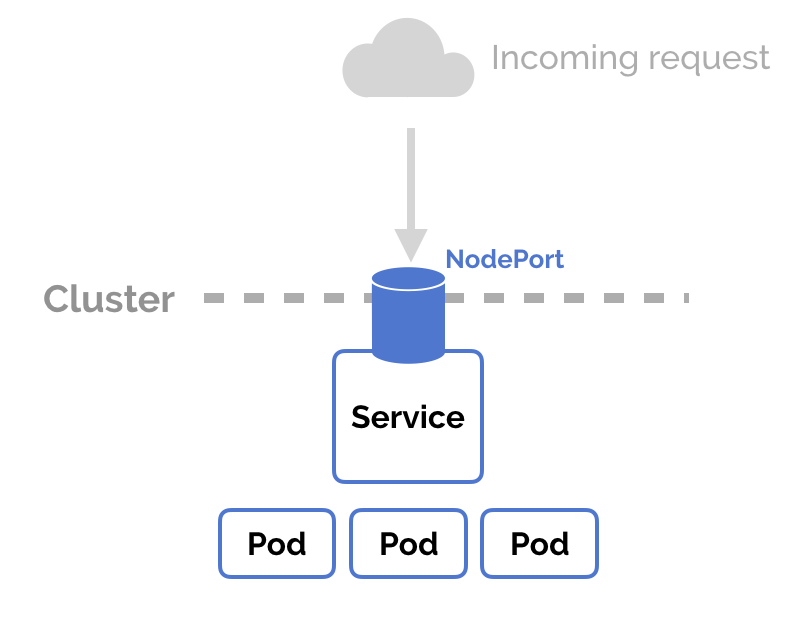
\includegraphics[totalheight=0.25\textheight]{service}
		\caption{Kubernetes service \cite{Service}}
	\end{center}
\end{figure}
\subsection{Ingress network}
An ingress network exposes the services in the cluster to the outside network i.e. to the clients. An ingress helps us in handling the outside traffic and routing it based on the context.\\
\begin{figure}[h!]
	\begin{center}
		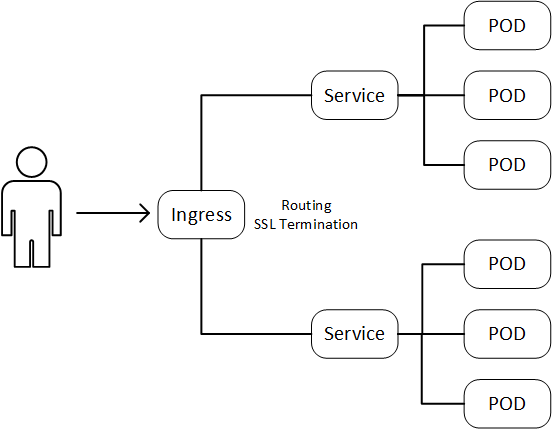
\includegraphics[totalheight=0.31\textheight]{ingress}
		\caption{Ingress network \cite{Ingress}}
	\end{center}
\end{figure}
\section{Networking in Kubernetes}
Kubernetes supports a large number of network plugins using different protocols. The type of networking to be used completely depends on the type of cluster you want to set up and your cluster requirements.\\\\
In a kubernetes network, each pod is assigned its own IP address. Pods can communicate with pods, nodes and services in a node without NAT. \\\\
The networking in kubernetes can be primarily broken down into 4 parts :
\begin{enumerate}
	\item Container to container communication
	\item Pod to pod communication
	\item Pod to service communication
	\item Service to external Communication
\end{enumerate}
The major plugins used for achieving these communications are :
\subsection{Flannel}
Flannel is the simplest kubernetes network  which satisfies all kubernetes requirements. Flannel is basically an overlay network.
\begin{figure}[h!]
	\begin{center}
		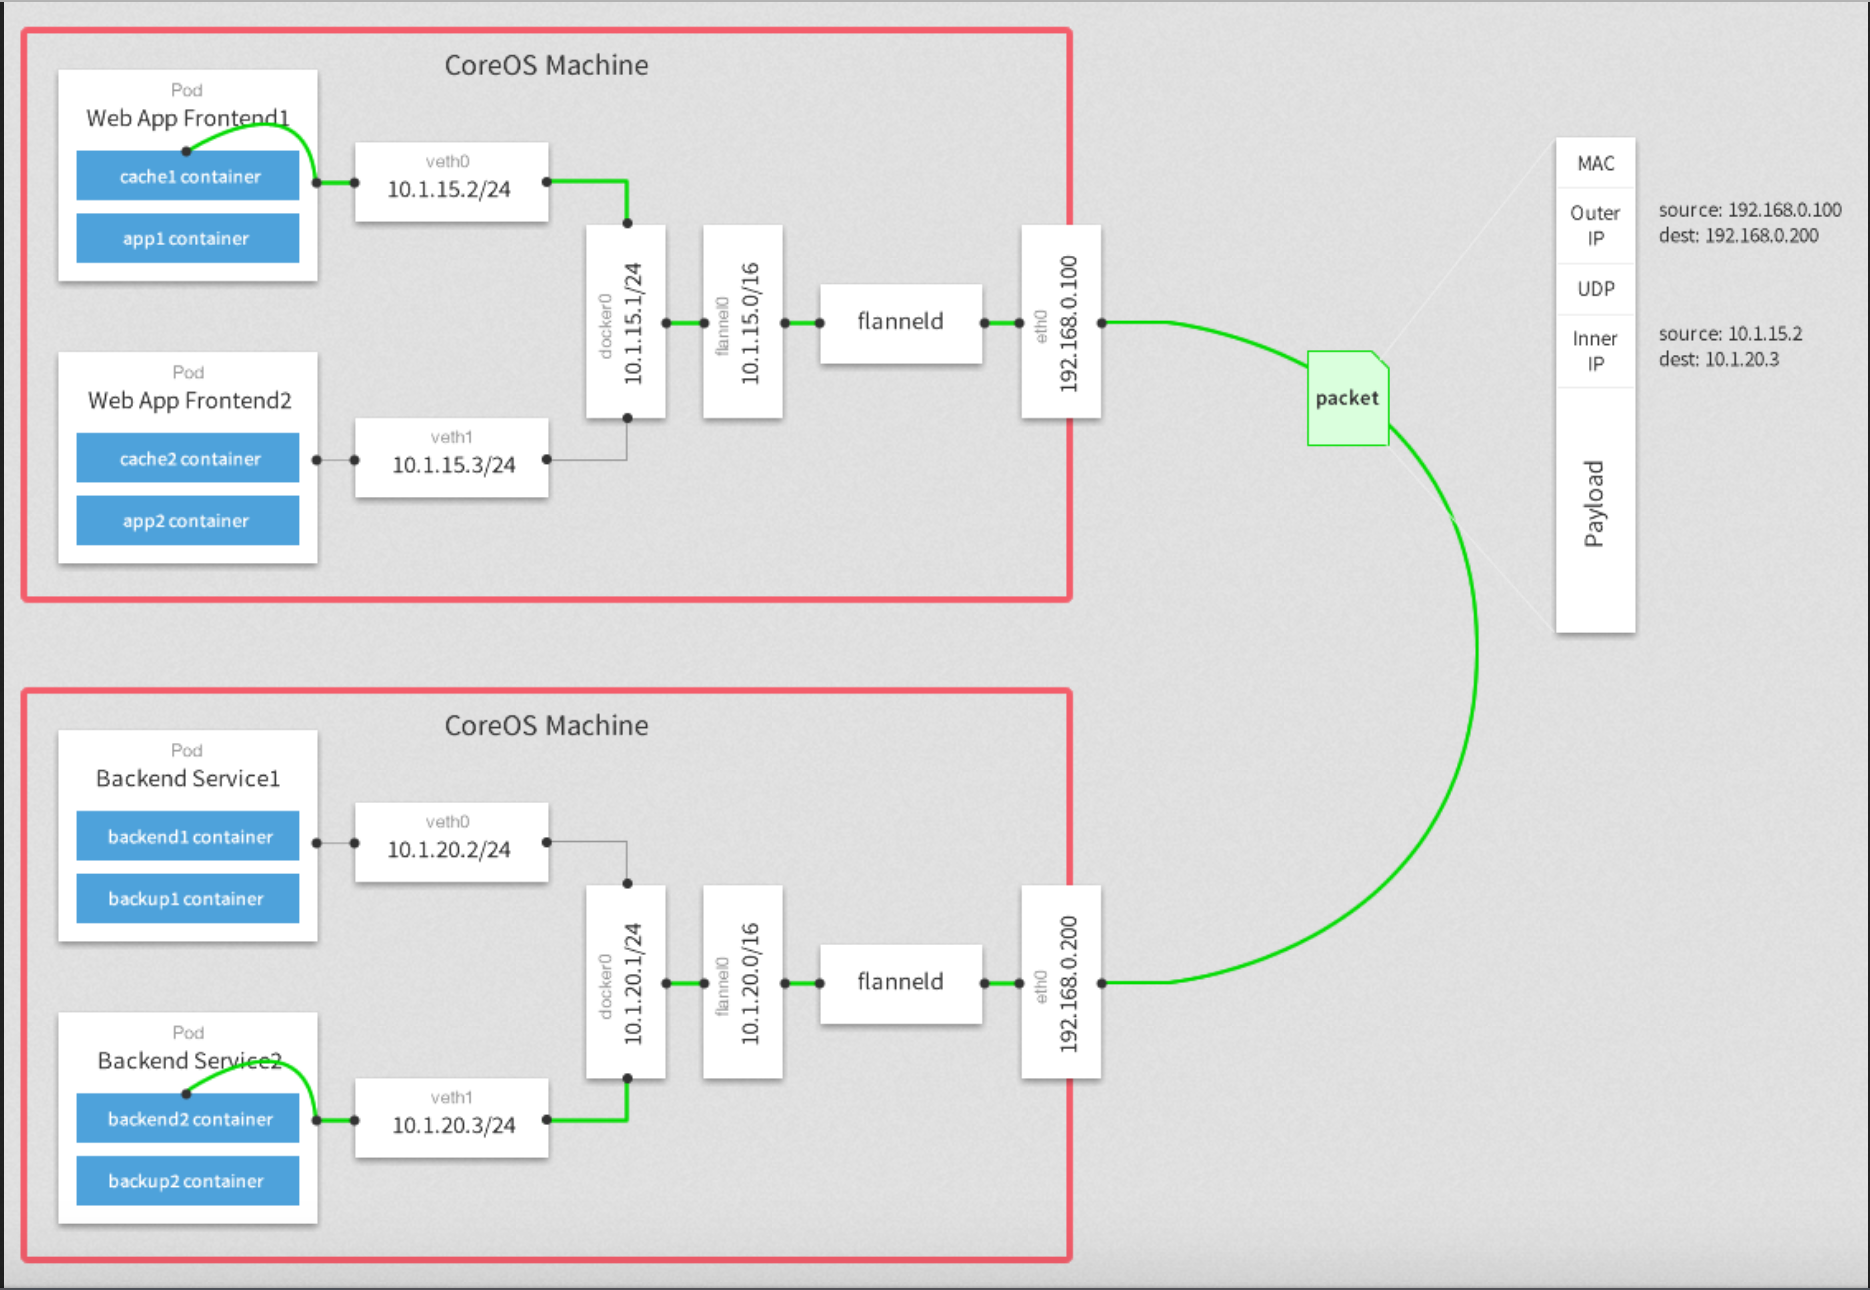
\includegraphics[totalheight=0.4\textheight, width=\textwidth]{flannel}
		\caption{Flannel network \cite{Flannel}}
	\end{center}
\end{figure}
\subsection{Calico}
Calico provides a highly scalable networking and network policy solution for connecting Kubernetes pods based on the same IP networking principles as the internet, for both Linux and Windows. Calico can be deployed without encapsulation or overlays to provide high-performance, high-scale data center networking.\\
\begin{figure}[h!]
	\begin{center}
		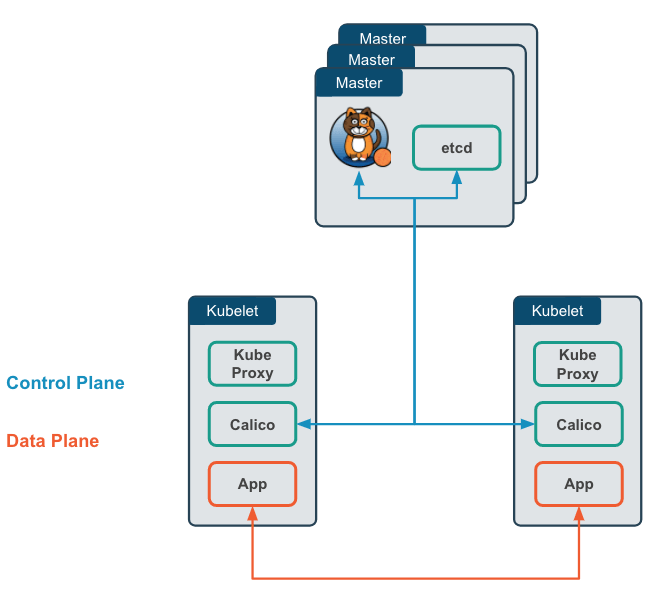
\includegraphics[totalheight=0.42\textheight]{calico}
		\caption{Calico network \cite{Calico}}
	\end{center}
\end{figure}

\subsection{Weavenet}
Weavenet is a simple network for kubernetes and its hosted applications. Weave Net runs as a CNI plug-in or stand-alone.
\begin{figure}[h!]
	\begin{center}
		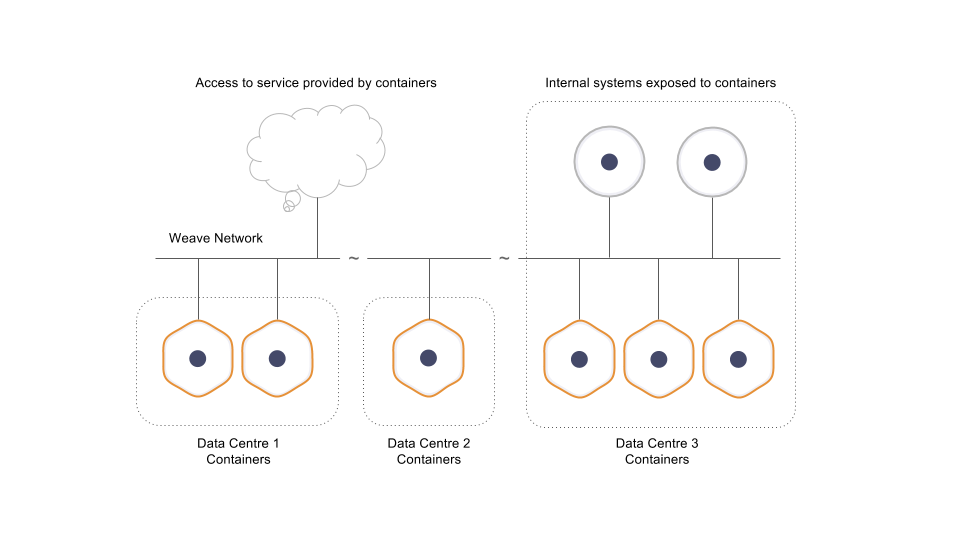
\includegraphics[totalheight=0.33\textheight]{weavenet}
		\caption{Weavenet \cite{Weavenet}}
	\end{center}
\end{figure}
\\\\\\\\\\\\\\\\\\\\\\\\
\\In addition to these, kubernetes supports many other plugins too. A list of them can be found in the official documentation page of kubernetes (\href{https://kubernetes.io/docs/concepts/cluster-administration/networking/}{Networking in Kubernetes})\cite{Knet}.
\section{Prerequisites for running kubernetes \cite{Prereq}}
\subsection{Disable Swap Space}
In order to set up a kubernetes cluster, all nodes including the master must have swap space disabled.
\begin{itemize}
	\item To disable swap space for currenThere are a lot of plugins available that can be used as per the requirements. In this project, we have used a calico pod network as CNI.\\\\t session, run: \\
	\textbf{\$ sudo swapoff -a}
	\item To permanently disable swap space, go to /etc/fstab and comment the swap space line.
\end{itemize}
\subsection{Make IP static}
All nodes in cluster including master must have a static IP address.\\
In order to manually make the IP static add the following lines to the file /etc/network/interfaces:\\\\
auto wlo1\\
iface wlo1 inet static\\
address  YOUR\_IP\_ADDRESS
\section{Kubernetes setup}
\begin{enumerate}
	\item Install docker (follow the steps given \hyperref[sec:dockerinstall]{here} to successfully install docker).
	\item Enable docker to run automatically on startup:\\
	\textbf{\$ sudo systemctl enable docker}
	\item Install curl:\\
	\textbf{\$ curl -s https://packages.cloud.google.com/apt/doc/apt-key.gpg $\vert$ sudo apt-key add}
	\item Add Google’s kubernetes repository:\\
	\textbf{\$ sudo apt-add-repository "deb http://apt.kubernetes.io/ kubernetes-xenial main"}
	\item Install kubeadm, kubectl and kubelet:\\
	\textbf{\$ sudo apt-get install kubeadm}\\
	\textbf{\$ sudo apt-get install kubectl}\\
	\textbf{\$ sudo apt-get install kubelet}
\end{enumerate}
\section{Setting up your Kubernetes cluster}
In order to set up your cluster first, initialise your master with kubeadm:\\\\
\textbf{\$ kubeadm init  -{}-apiserver-advertise-address=YOUR\_IP\_ADDRESS    -{}-pod-network-cidr=40.196.0.0/16}\\\\
On successful execution of the command, we get a join command for the worker nodes to join the cluster. Preserve this command to bring nodes into the cluster once the dashboard is created.\\\\
You can also generate the join token by running the command :\\\\
\textbf{\$ kubeadm token create}\\\\
And the SHA256 key can be generated by running the command:\\\\
\textbf{\$ openssl x509 -pubkey -in /etc/kubernetes/pki/ca.crt $|$ openssl rsa -pubin -outform der 2$>$/dev/null $|$ openssl dgst -sha256 -hex | sed 's/\string^.* //'}\\\\
Now to bring any node into the cluster run the following command into the cluster after changing the IP with your master system’s IP address, token and SHA256 key with that generated by running the above command:\\\\
\textbf{\$ kubeadm join IP\_OF\_MASTER:6443 -{}-token GENERATED\_TOKEN -{}-discovery-token-ca-cert-hash sha256:GENERATED\_HASH}\\\\
Once the cluster has been successfully initialised, run the following commands :\\\\
\textbf{
	\$ mkdir -p \$HOME/.kube\\
	\$ sudo cp -i /etc/kubernetes/admin.conf \$HOME/.kube/config\\
	\$ sudo chown \$(id -u):\$(id -g) \$HOME/.kube/config
}
\subsection{Setting up a pod network}
There are a lot of plugins available that can be used as per the requirements. In this project, we have used a calico pod network as CNI.\\
Once the network is set up, we need to install and host the dashboard on localhost.Flannel is a overlay network whereas calico is an L3 network. The advantages in detail can be read from this  \href{https://medium.com/@jain.sm/flannel-vs-calico-a-battle-of-l2-vs-l3-based-networking-5a30cd0a3ebd}{medium Blog}.\\\\
i) To install and set up a calico pod network, run the command :\\\\
\textbf{\$ kubectl apply -f https://docs.projectcalico.org/v3.1/getting-started/kubernetes/\\installation/hosted/kubeadm/1.7/calico.yaml}\\\\
ii) To install and set up flannel pod network, run the command :\\\\
\textbf{\$ sudo kubectl apply -f https://raw.githubusercontent.com/coreos/flannel/master/\\Documentation/kube-flannel.yml}\\\\
Run \textbf{kubectl get pods -o wide --all-namespaces} to view all the running pods:\\\\
In case you face a CrashLoopBackOff error in running the coredns pods. Resolve the issue using the stackoverflow link \href{https://stackoverflow.com/questions/53075796/coredns-pods-have-crashloopbackoff-or-error-state/53414041#53414041}{https://stackoverflow.com/questions/53075796/coredns-pods-have-crashloopbackoff-or-error-state/53414041\#53414041}\cite{Coredns} \\\\
Once the network is set up, we need to install and host the dashboard on localhost.
\subsection{Setting up and hosting the dashboard \cite{Dashboard}}
i) For installation and hosting in localhost : \\\\
\textbf{\$ kubectl create -f https://raw.githubusercontent.com/kubernetes/dashboard/\\v1.8.3/src/deploy/recommended/kubernetes-dashboard.yaml}\\\\
ii) For Creating service account:\\\\
\textbf{\$ kubectl create serviceaccount dashboard -n default}\\\\
iii) To add cluster binding rules to the dashboard:\\\\
\textbf{\$ kubectl create clusterrolebinding dashboard-admin -n default 
	\\-{}-clusterrole=cluster-admin 
	\\-{}-serviceaccount=default:dashboard}\\\\
iv) To generate token for login\\\\
\textbf{\$ kubectl get secret \$(kubectl get serviceaccount dashboard\\ -o jsonpath="{.secrets[0].name}") -o jsonpath="{.data.token}" $|$ base64 -{}-decode}\\\\
After the token is generated you can run the dashboard on localhost on port 8001(default). To bring up the dashboard run the command :\\\\
\textbf{\$ kubectl proxy}\\\\
Now you can visit the dashboard on the localhost:8001 at url:\\\\
\href{http://localhost:8001/api/v1/namespaces/kube-system/services/https:kubernetes-dashboard:/proxy/}{http://localhost:8001/api/v1/namespaces/kube-system/services/https:kubernetes-\\dashboard:/proxy/}\\\\
The dashboard can be accessed by entering the token generated. We can see the pods running, deployments, services and volumes created. We can also scale up and scale down the number of replicas.
\subsection{Kubernetes commands for getting resource info}
In order to get the complete details of  the pods via command line run the command :\\\\
\textbf{\$ kubectl get pods -o wide -{}-all-namespaces}\\\\
For viewing pods in default namespace run the command:\\\\
\textbf{\$ kubectl get pods}\\\\
Similarly for viewing deployments and services run the corresponding commands:\\\\
\textbf{\$ kubectl get deployments}\\
\textbf{\$ kubectl get services}\\\\
Once the cluster is set up, we can create deployments for the running in the cluster. We can expose these deployments to endpoints via services and to external traffic by creating an ingress network.
\section{Kubernetes API Server}
The Gateway to the Kubernetes cluster is the Kubernetes API server. It is a centralized system that is accessed by all users, automation, and components in the Kubernetes cluster. The API server implements a RESTful API over HTTP, performs all API operations, and is responsible for storing API objects into a tent storage backend.
\begin{figure}[h!]
	\begin{center}
		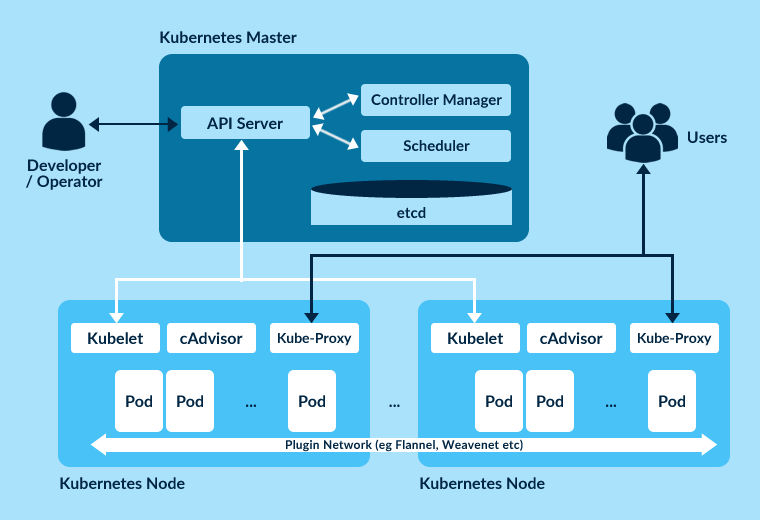
\includegraphics[totalheight=0.32\textheight]{kubernetesapiserver}
		\caption{Kubernetes architecture \cite{KArc}}
	\end{center}
\end{figure}
\\\\
\subsection{Pieces of API Server}
Kubernetes API server has three core functions:
\begin{itemize}
	\item \textbf{API management:}\\\\
	In API management process, APIs are exposed and managed by the server.
	\item \textbf{Request processing:}\\\\
	Request processing processes individual API requests from a client.
	\item \textbf{Internal control loops:}\\\\
	Internal control loops has internals responsibilities for background operations necessary to the successful operation of the API server.
\end{itemize}
\subsection{API Management \cite{KubernetesManagement}}
The API server is an HTTP server—thus, every API request is an HTTP request. But the characteristics of those HTTP requests must be described so that the client and server know how to communicate. For the purposes of exploration, it’s great to have an API server actually up and running so that you can poke at it. You can either use an existing Kubernetes cluster that you have access to, or you can use the minikube tool for a local Kubernetes cluster. To make it easy to use the curl tool to explore the API server, run the kubectl tool in proxy mode to expose an unauthenticated API server on localhost:8001 using the following command:\\\\
\textbf{\$ kubectl proxy}
\subsection{Request Management}
The main aim of the API server is to receive and process API calls in the form of HTTP requests.\\
Type of request performed by the API server are as follows:
\begin{itemize}
	\item GET
	\item LIST
	\item POST
	\item DELETE
\end{itemize}
\begin{figure}[h!]
	\begin{center}
		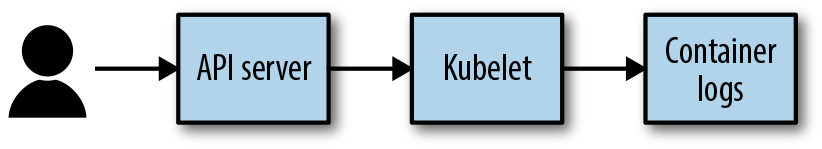
\includegraphics[totalheight=0.1\textheight]{kubereqman}
		\caption{Request management \cite{Request}}
	\end{center}
\end{figure}
\section{ETCD}
A key-value storage for kubernetes backing store for all cluster data.
\section{Kube-Scheduler}
If there is a newly created pod which is not allocated any node then Kube-Scheduler select a node for them to run.
\section{Kube-Control-Manager}
Kube-Control-Manager is a component on master that runs controllers.
Each controller is a separate process but they are all merged.\\\\
These controllers include:
\begin{itemize}
	\item \textbf{Node controller:} Responsible for noticing and responding when nodes go down.
	\item \textbf{Replication controller:} Responsible for maintaining the correct number of pods for every replication controller object in the system.
	\item \textbf{Endpoints controller:} Populates the Endpoints object (that is, joins Services \& Pods).
	\item \textbf{Service Account \& Token Controllers:} Create default accounts and API access tokens for new namespaces.
\end{itemize}
\section{Converting docker-compose file to its Kubernetes equivalent}
As we have docker-compose in docker we similarly have a kompose file with kubernetes. We can deploy a docker-compose created stack on a docker-swarm cluster. 
\subsection{Kompose}
Kompose is tool provided by kubernetes which converts a docker-compose file into kompose files for providers like kubernetes and openshift. For each service in a compose file we have a deployment, service and persistent volume claim file in kompose. We can also create our persistent volume file is we require a persistent volume for our services.\\\\
\textbf{Installing Kompose on Linux :}
\begin{enumerate}
	\item Download the latest release and install in the system:\\\\
	\textbf{\$ curl -L https://github.com/kubernetes/kompose/releases/download/\\v1.17.0/kompose-linux-amd64 -o kompose}
	\item Give executable permission and move the directory:\\\\
	\textbf{\$ chmod $+$x kompose\\
		\$ sudo mv ./kompose /usr/local/bin/kompose}
\end{enumerate}
In order to convert the compose file into kompose run the command :\\\\
\textbf{\$ kompose convert -f docker-compose.yml}\\\\
In order to run yaml file in kubernetes we use the command :\\\\
\textbf{\$ kubectl apply -f FILE\_NAME.yaml}\\\\
Kompose provides an easy solution for  converting a docker-compose file into kompose. Docker-compose is an easy to write file whereas kompose files are a bit lengthy and it get a bit tedious to code. So kompose provides an easy alternative. The files provided by kompose does not have a 100\% conversion rate but we can change files as per our requirements.\\\\
We have converted the docker-compose.yml and docker-compose-host.yml file in devstack to kompose file. We have created a PersistentVolume.yml for each service which creates a pool of space from where a persistentvolumeclaim can claim a volume for the pod. The kompose converts the file in kompose objects and then into kuebernetes objects and then into yaml or json output as per our requirements.
\begin{figure}[h!]
	\begin{center}
		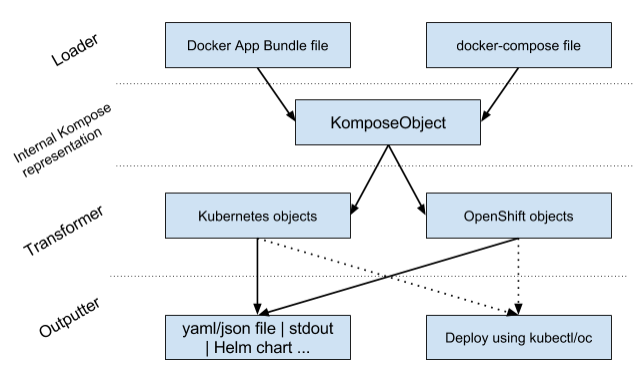
\includegraphics[totalheight=0.38\textheight]{kompose}
		\caption{Kompose \cite{Kompose}}
	\end{center}
\end{figure}\\\\\\\\\\
\\The persistent volumes present are created by admin so that a developer can attach a claim and use the volume for the pod.
\begin{figure}[h!]
	\begin{center}
		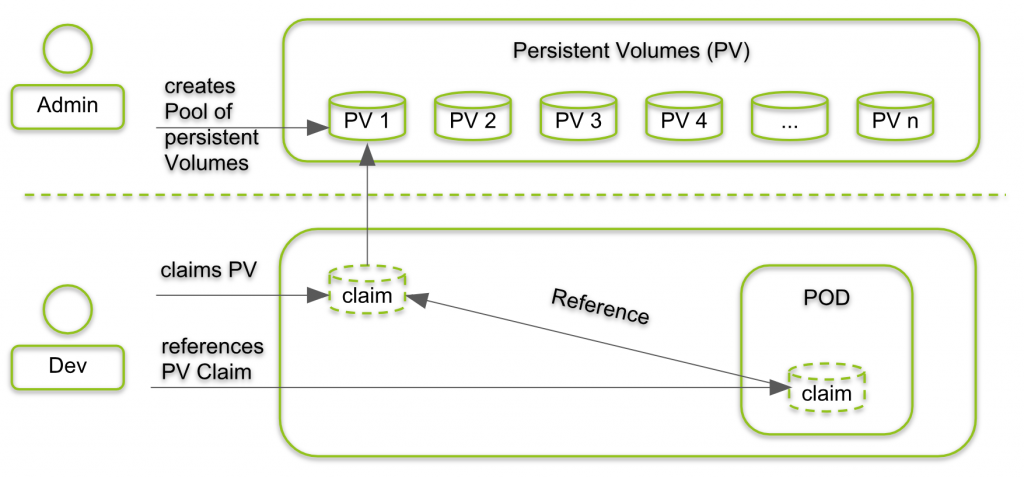
\includegraphics[totalheight=0.33\textheight]{persistentvolumes}
		\caption{Persistent volumes \cite{Persistent}}
	\end{center}
\end{figure}
\subsection{Compose on Kubernetes}
We also have a tool compose-on-kubernetes provided by docker which converts a docker-compose file into compose file. It is an open source tool and can be explored to check its accuracy and efficiency.(\href{https://github.com/docker/compose-on-kubernetes.git}{https://github.com/docker/compose-on-kubernetes.git})\\\\
In order to deploy services on a stack using Kubernetes as an orchestrator, we can use Compose on Kubernetes. In order to install Compose on Kubernetes on a global Kubernetes engine, follow the link \url{https://github.com/docker/compose-on-kubernetes/blob/master/docs/install-on-gke.md}
\chapter{Our progress}
In this project, our aim was to deploy an instance of Open edX on a Kubernetes cluster.
\section{Kubernetes cluster}
At first, we set up a Kubernetes cluster as mentioned above with one master and three nodes.
\begin{figure}[h!]
	\begin{center}
		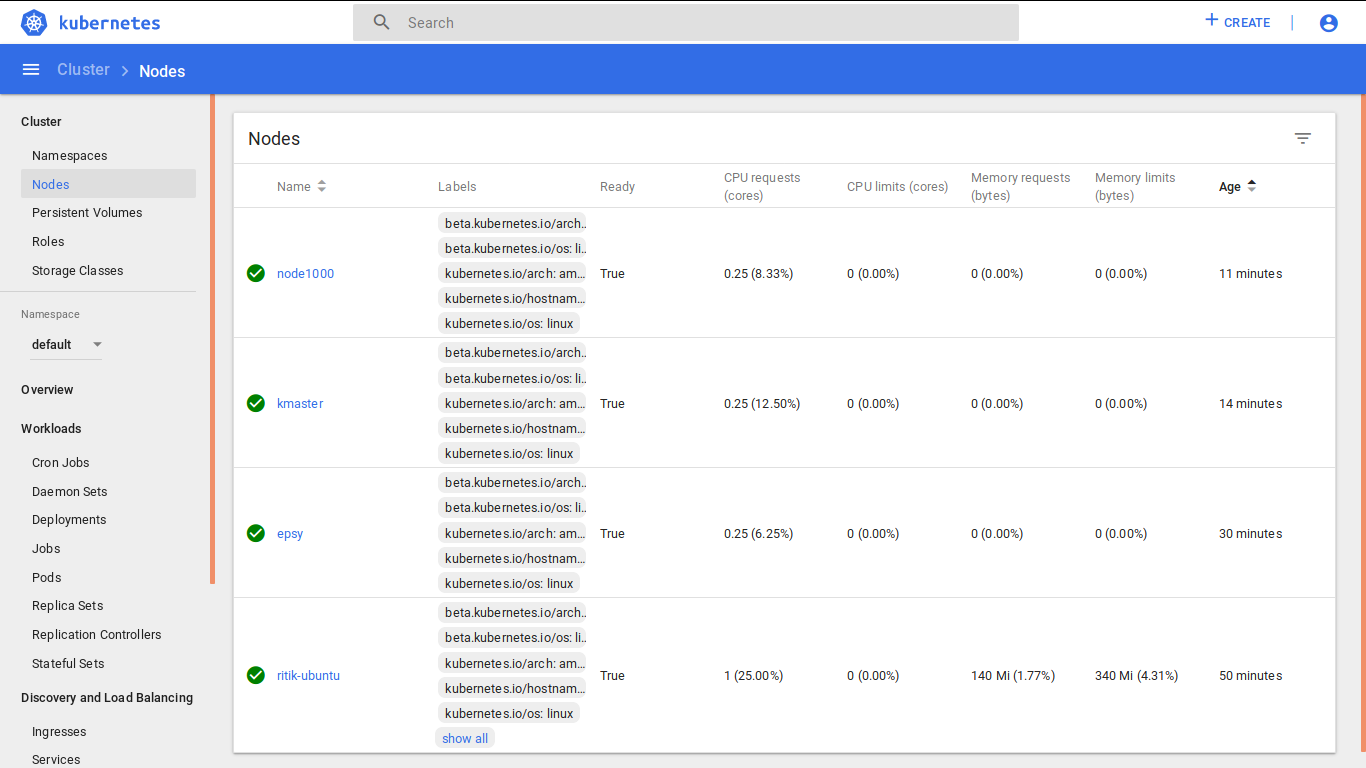
\includegraphics[totalheight=0.4\textheight]{cluster}
		\caption{Nodes connected in a Kuberentes cluster}
	\end{center}
\end{figure}
\\\\\\
\section{Kompose}
We converted the docker-compose.yaml file for Open edX containers to multiple Kubernetes deployment files (YAML). But, since the conversion rate was not 100\%, we had to create persistent volumes and claims for those volumes on our own.\\\\
The converted files can be found in the github repository : \\ \href{https://github.com/fresearchgroup/Configurable-and-Scalable-IITBombayX-MOOC-platform-on-Commodity-Servers/tree/master/kompose_files}{https://github.com/fresearchgroup/Configurable-and-Scalable-IITBombayX-MOOC-platform-on-Commodity-Servers/tree/master/kompose\_files} \cite{Komposefiles}
\section{Persistent volumes and Persistent volume claims}
We made YAML files to create persistent volumes and then attached each volume to a claim using its corresponding persistent-volume-claim.yaml file.\\\\
The persistent volume and claim files can be found in the github repository :\\\\ \href{https://github.com/fresearchgroup/Configurable-and-Scalable-IITBombayX-MOOC-platform-on-Commodity-Servers/tree/master/host_volumes}{https://github.com/fresearchgroup/Configurable-and-Scalable-IITBombayX-MOOC-platform-on-Commodity-Servers/tree/master/host\_volumes} \cite{Hostvolumes}. \\\\You need not create all the persistent volume and claim files manually, we have created a bash script \textbf{volumes.sh} in the same directory that does the job. 
\begin{figure}[h!]
	\begin{center}
		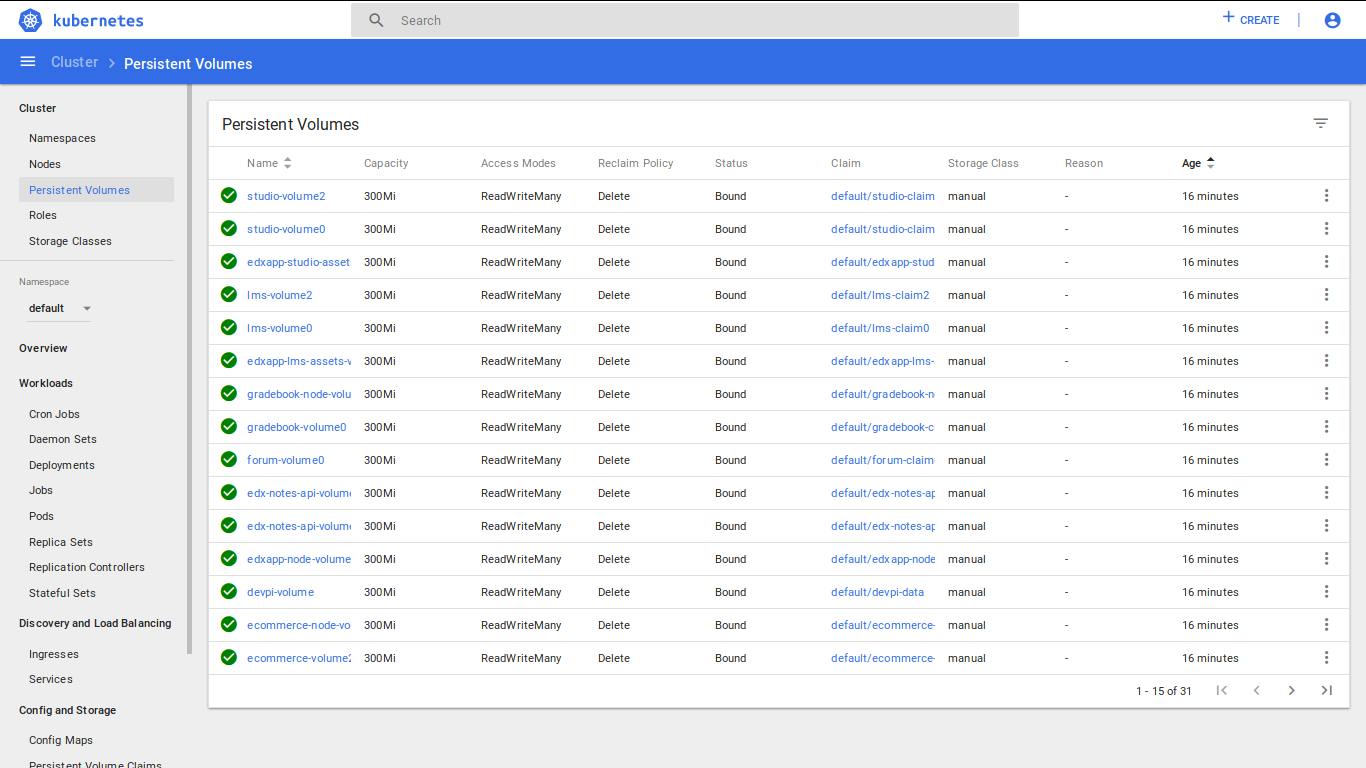
\includegraphics[totalheight=0.39\textheight]{PersistentVolume}
		\caption{Persistent Volumes}
	\end{center}
\end{figure}
\begin{figure}[h!]
	\begin{center}
		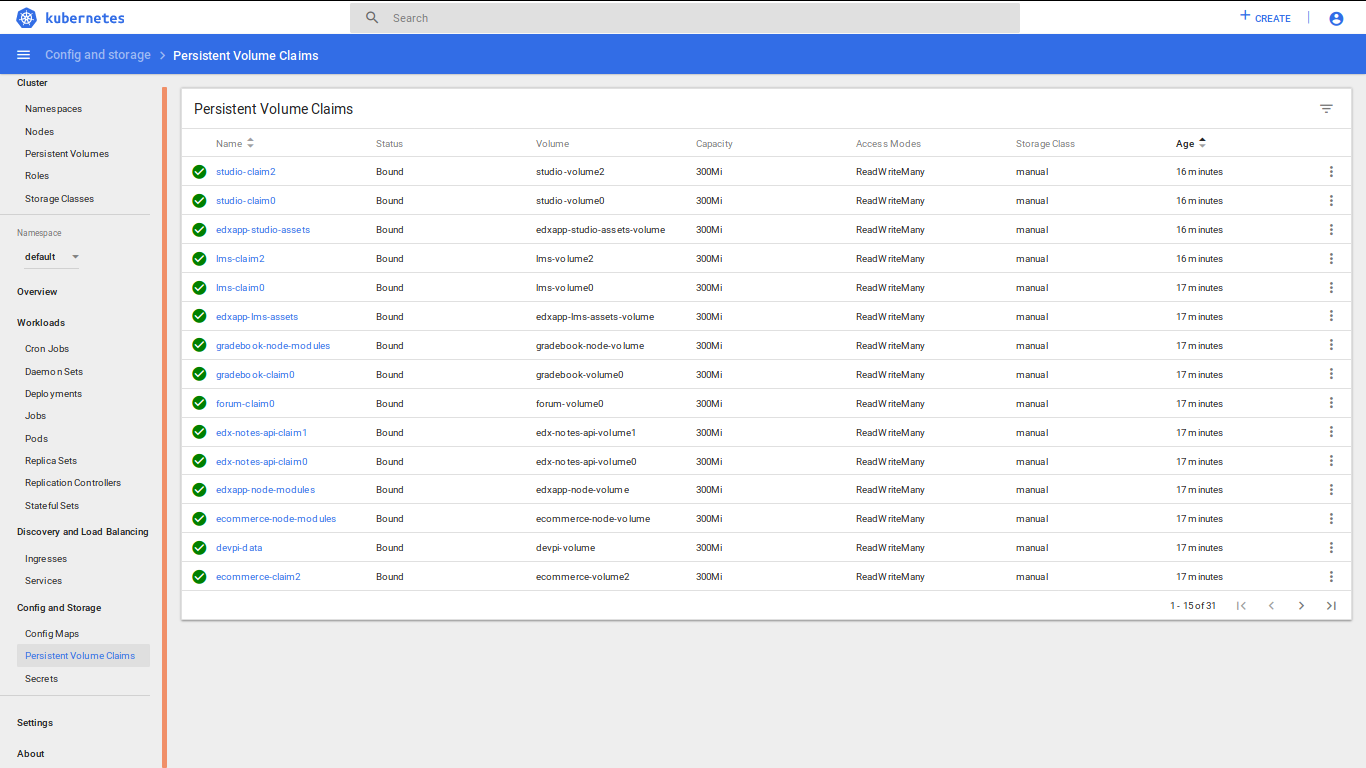
\includegraphics[totalheight=0.39\textheight]{PersistentVolumeClaim}
		\caption{Persistent Volume Claims}
	\end{center}
\end{figure}
\section{Kubernetes deployment}
We then deployed all the 15 containers on the cluster. Kubernetes assigned the appropriate node (one among the two) for each container to run.
\begin{figure}[h!]
	\begin{center}
		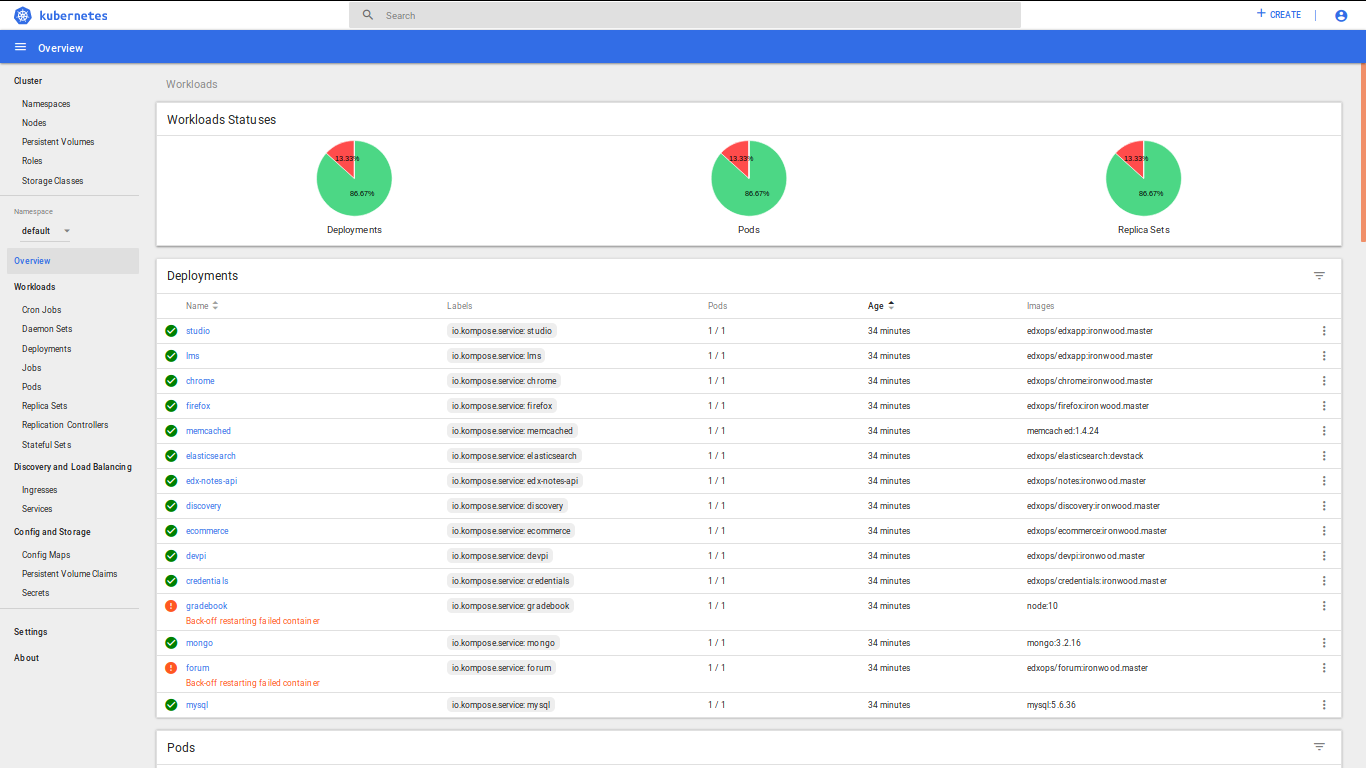
\includegraphics[totalheight=0.34\textheight]{fgcrash}
		\caption{Kubernetes deployments}
	\end{center}
\end{figure}
\\The gradebook and forum deployments were unsuccessful. But, those two are not necessary for running the bare minimum Open edX instance and hence can be removed:
\begin{figure}[h!]
	\begin{center}
		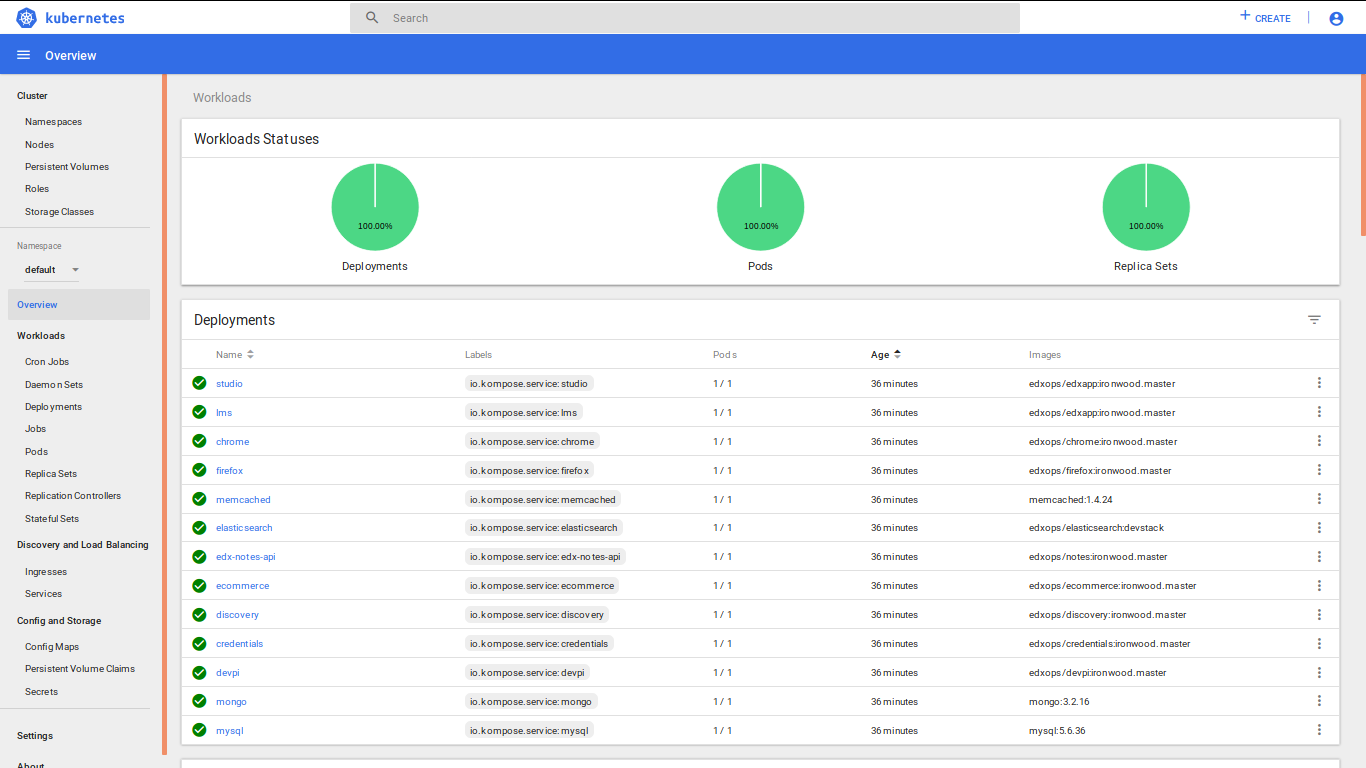
\includegraphics[totalheight=0.34\textheight]{dep100}
		\caption{Kubernetes deployments after removing gradebook and forum}
	\end{center}
\end{figure}
\section{Fault handling}
We removed one node from the cluster and found out that Kubernetes deployed all the containers running on that node to the node that was still a part of the cluster.\\\\
\textbf{The pods running in the cluster:}
\begin{itemize}
	\item Before deleting the node epsy: 
		\begin{figure}[h!]
			\begin{center}
				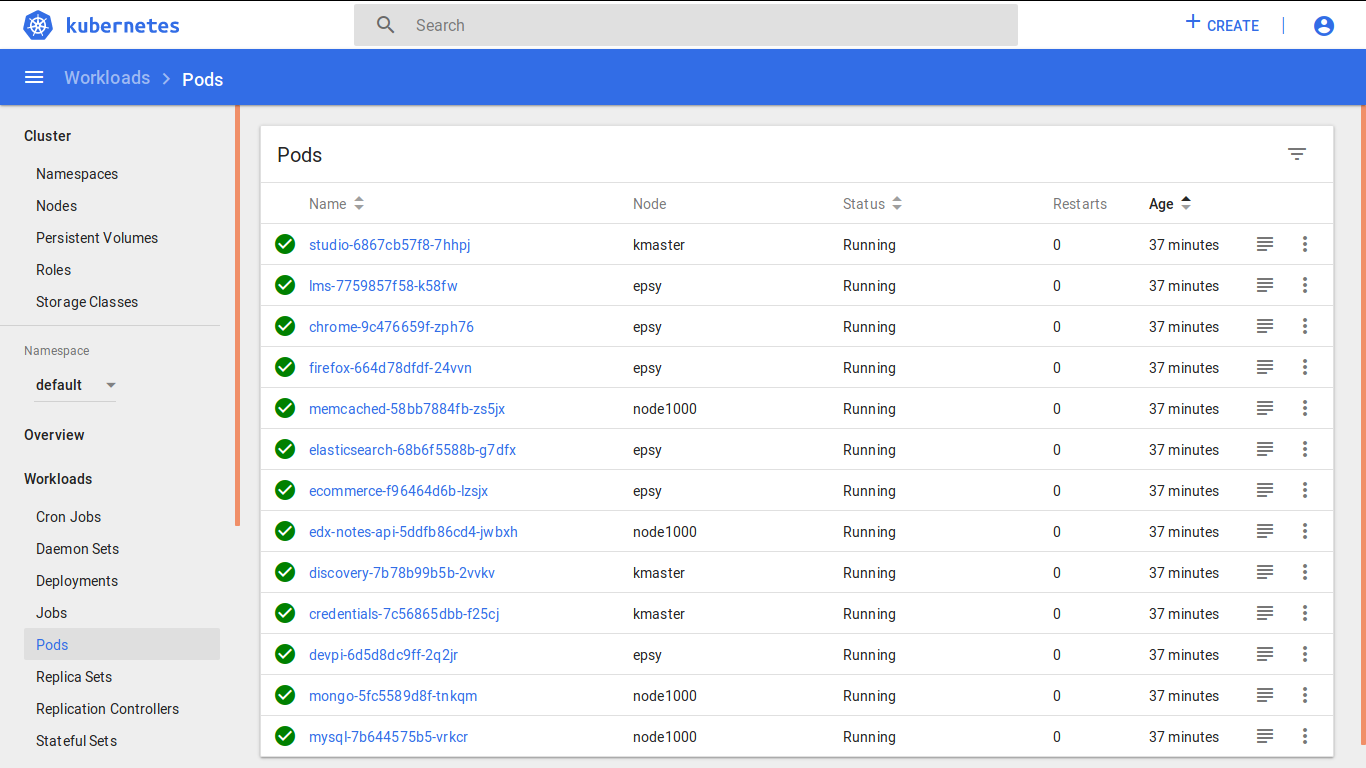
\includegraphics[totalheight=0.32\textheight]{podswithepsy}
				\caption{Pods running before deleting a node}
			\end{center}
		\end{figure}
	\item After deleting the node epsy:
		\begin{figure}[h!]
			\begin{center}
				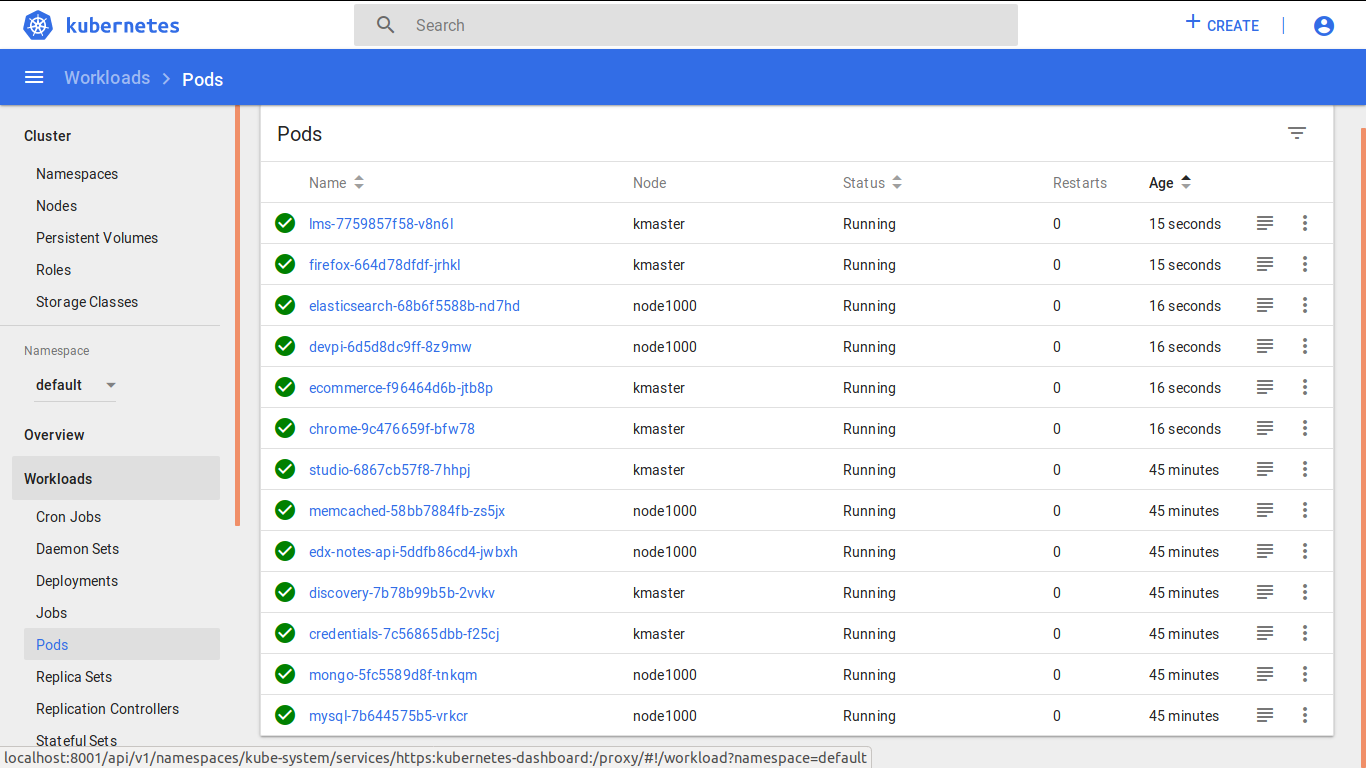
\includegraphics[totalheight=0.32\textheight]{podswithoutepsy}
				\caption{Pods running after deleting the node}
			\end{center}
		\end{figure}
\end{itemize}
As we can see, the pods which were earlier running on the node epsy, now run on the remaining nodes after, their host node is deleted. This rescheduling of the pods is done automatically by Kubernetes once a node goes down. The reshudiling takes very less time as is clear from the image (15-16 seconds in this case). 
\\\\\\\\\\
\section{Provisioning}
The file provision.sh in the devstack directory has the commands and links to the files that are to be executed for provisioning and migration of databases. Those are simply docker commands. Since, our containers are running on a Kubernetes cluster, we used the \textbf{kubectl exec} in place of \textbf{docker exec} to run commands inside the containers. But we faced an internet connectivity issue for the pods: \\\\
\textbf{The containers running inside the Kubernetes cluster were not able to connect to the internet}\\\\
Commands those were to be executed inside a container and required internet access failed, as containers were not able to connect to the internet.\\\\
\textbf{Suggested resolutions:\\\\}These are some methods that may solve this issue (due to lack of time, we were not able to try them properly and anyone taking up this project from here on can try these methods):
\begin{itemize}
	\item On further research, we found out that the internet connectivity problem of the containers was probably due to some issue in the DNS resolution. This can be further looked up using this link: \href{https://blog.yaakov.online/kubernetes-getting-pods-to-talk-to-the-internet/}{https://blog.yaakov.online/kubernetes-getting-pods-to-talk-to-the-internet/}\cite{DNS}
	\item We can mention the commands that are to be executed inside a containere inside its deployment file itself. This is probably a better way than the above one as here the commands will be executed inside any new container that is created through that deployment file. This can be done by using \textbf{command} and \textbf{args} fields in the deployment file.\\\\
	We can create a ConfigMap containing all the arguments to be passed to the commands that are to be run inside the container. So, whenever a new pod is created, the containers are configured accordingly.\cite{Configmap}
	\item If we have an already running instance of Open edX devstack version on a machine, then we can use the command \textbf{docker commit} to create a new image that reflects the changes made on the container while provisioning and then use the new image for deployment purpose in our Kubernetes cluster.
\end{itemize}
\pagebreak
\chapter{Performance Testing Open edX Ironwood Release}
Given a certain load, Performance Testing allows us to determine and examine non-functional parameters like speed and stability of an application.
\par
\section{Tools used for Performance Testing}
JMeter is a popular tool used for performance testing. Apart from being an open-source software, JMeter is purely written in Java and hence, is platform independent. Also, it provides a GUI to easily set up a test plan. This, combined with the support for a full multithreading framework and the ability to test a wide range of protocols and applications, makes it a very good tool for performance testing.
\par
One can install JMeter by downloading the required binaries from
\\
\url{https://jmeter.apache.org/download_jmeter.cgi}.
\par
\section{JMeter Test Scripts}
A JMeter test script is a collection of user activities that have been pre-recorded using a proxy. These scripts are stored in the XML format with $.jmx$ extension.
\par
The test script can be recorded as follows:\cite{Performance}
\begin{enumerate}
	\item Firstly, create a new test plan. A test plan describes what JMeter should do when we run a test script. 
	\item Next, right-click on the newly created test plan and add a thread group. (Add-$>$Threads (Users)-$>$Thread Group) A thread group is used to simulate users for testing an application.
	\item Add an instance of the HTTP(S) Test Script Recorder via the add sub-menu accessed by right-clicking on the test plan. (Add-$>$Non-Test Elements-$>$HTTP(S) Test Script Recorder)
	\item In the recorder instance created in the previous step, set the Target Controller field to the newly created Thread Group. This field can be accessed in the Test Plan Creation tab.
	\item Thereafter, configure the port field to an unused port on your system.
	\item We must instruct the recorder to bypass recording the loading of static elements like images. To do this, go to the request tab in the recorder instance created earlier, and click on the Add Suggested Excludes button to add default static files' extensions. This can be modified as per convenience. 
	\item Since a user may pause for a while between successive requests, the need to add think time to our test script is evident. JMeter provides various timers. We will use a Uniform Random Timer here, which can be added to the HTTP(S) Test Script Recorder instance. With each timer, we associate some parameters. For a Uniform Random Timer, these are Random Delay Maximum and Constant Delay Offset. This timer samples a point from a Uniform Probability Distribution such that it lies between 0 and the Random Delay Maximum value. Thereafter, it adds the Constant Delay Offset to it. To modify the Constant Delay Offset value, use \$\{T\} in the corresponding field. 
	\item JMeter would now act as an HTTP proxy and would listen to all the incoming and outgoing requests on the configured port.
	\item Now, we configure the proxy settings in the browser to send requests to the JMeter proxy.
	\item Click on the Start button available in the State tab in the recorder instance to start the recording.
	\item Note that the JMeter Root CA certificate must be installed in the web browser to record encrypted web requests. 
	\item To do this, go to the bin directory in the JMeter directory to locate the file named ApacheJMeterTemporaryRootCA, and install it in the system as well as the browser being used for recording the test script. In Firefox, for example, one needs to go to the options page, move to the Privacy and Security tab, click on the View Certificates button, and then click on the Import button to add the JMeter's self-signed certificate.
	\item Once the recording starts, execute the test scenario.
	\item Thereafter, click on the Stop button in the Transaction Controller to stop the recording.
\end{enumerate}
\par
\section{Viewing JMeter Test Results using Listeners}
JMeter listeners enable us to view and analyze the test results in graphical or tabular form. Some of these are:
\begin{itemize}
	\item View Result Tree: This listener allows us to view a tree of samples' responses with their response codes. Furthermore, the response of each sample is shown separately.
	\item Summary and Aggregate Report: These listeners give an abridged view of information like Request Count, Average, Median, Min, Max, 90\% Line, Error Rate, Throughput, Requests/second, and KB/sec for each uniquely named sample in the test plan. For low memory consumption, the Summary Report listener can be a good alternative.
\end{itemize}
\par
Due to insufficient Java Heap Space, a test plan execution may result in JMeter giving an Out of Memory error. To resolve this, edit the jmeter.bat (for Windows) or jmeter.sh (for Linux) files and update the JVM\_ARGS parameter accordingly.
\\
\par
\section{Test Scenario}
Our test scenario is as follows:
\begin{enumerate}
	\item The user registers on the website.
	\item The user views a list of available courses.
	\item The user chooses a test course.
	\item The user enrolls in the chosen course.
	\item The user views the chosen course's dashboard.
	\item The user chooses the quiz modules.
	\item The user attempts the quiz.
	\item The user submits the quiz responses for evaluation.
\end{enumerate}
We had used this scenario since it involves all the activities that can be performed by a user on a course page.
\par
\section{Testing Open edX Native Installation}
\subsection{System Configurations}
Here are the details of the hardware and software configuration of the application under test and the client machine that has been used to generate load.
\subsection{Load Generator System Details}
\begin{itemize}
	\item Operating System: Windows 10 Home 64-bit
	\item RAM: 8GB
	\item Processor: Intel(R) Core(TM) i5-7200U CPU @ 2.50GHz x 2 Cores
\end{itemize}
\subsection{Server Configuration}
\begin{itemize}
	\item Operating System: Ubuntu 16.04.6 LTS
	\item RAM: 7.61 GB
	\item Processor: Intel Common KVM Processor @ 2.095 MHz x 2
\end{itemize}
\subsection{Test Details}
\begin{itemize}
	\item Duration: $1$ Hour
	\item Virtual Connections: 100
\end{itemize}

\subsection{Test Results}
The application under test could handle 100 users for the specified server configuration under the current test setup. Furthermore, the test fails for around 120-130 users.
\\\\\\\\\\\\\\\\\\\\\\
\begin{figure}[h!]
	\centering
	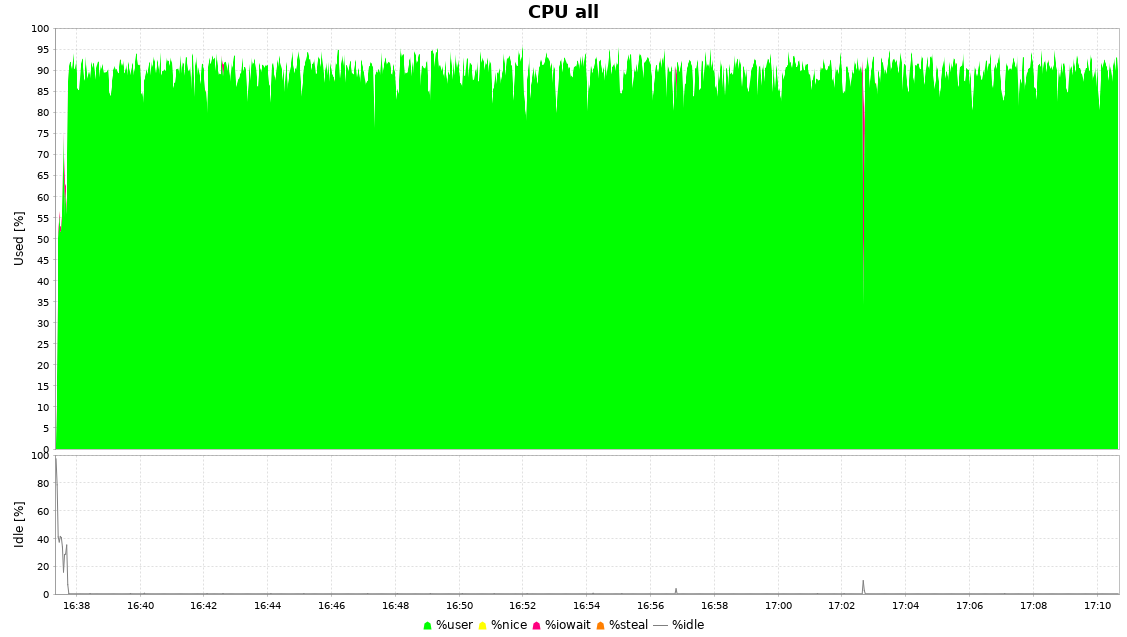
\includegraphics[width=\textwidth,height=\textheight,keepaspectratio]{intro/cpu_mridul.png}
	\caption{SAR CPU Metrics}
\end{figure}
\begin{figure}[h!]
	\centering
	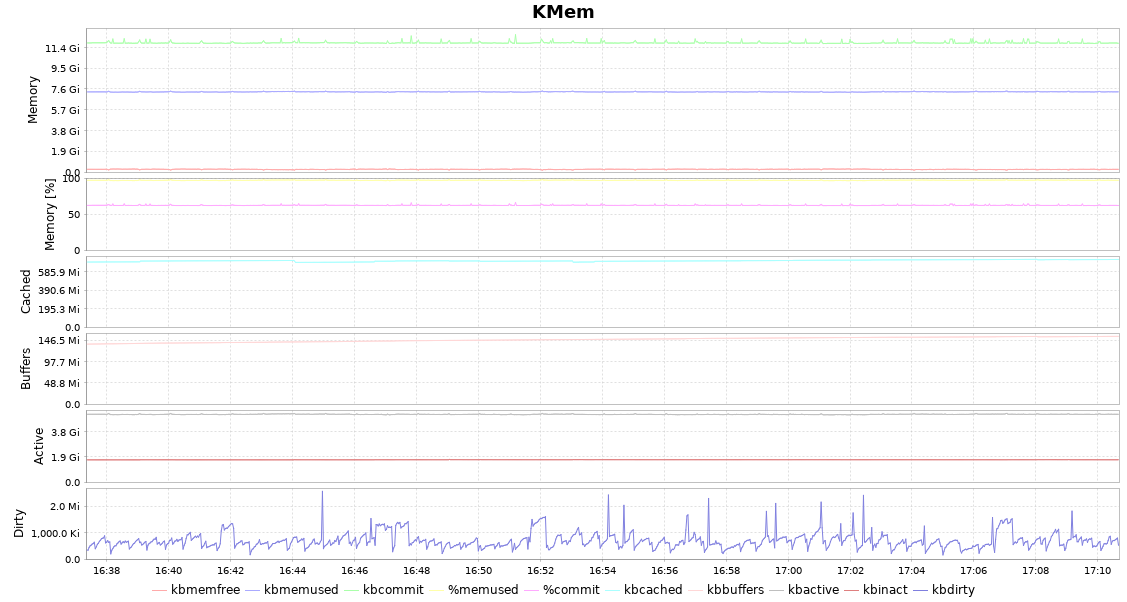
\includegraphics[width=\textwidth,height=\textheight,keepaspectratio]{intro/mem_mridul.png}
	\caption{SAR Memory Metrics}
\end{figure}

\newpage
\begin{figure}[h!]
	\centering
	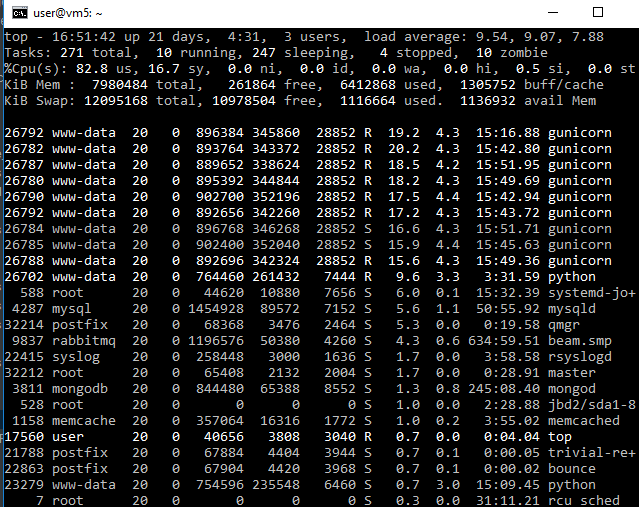
\includegraphics[width=\textwidth,height=\textheight,keepaspectratio]{intro/S1.png}
	\caption{A look at the top command, 15 minutes into the test. Guincorn, which is a Python Web Server Gateway Interface HTTP Server, takes up most of the CPU resources.}
\end{figure}
\begin{figure}[h!]
	\centering
	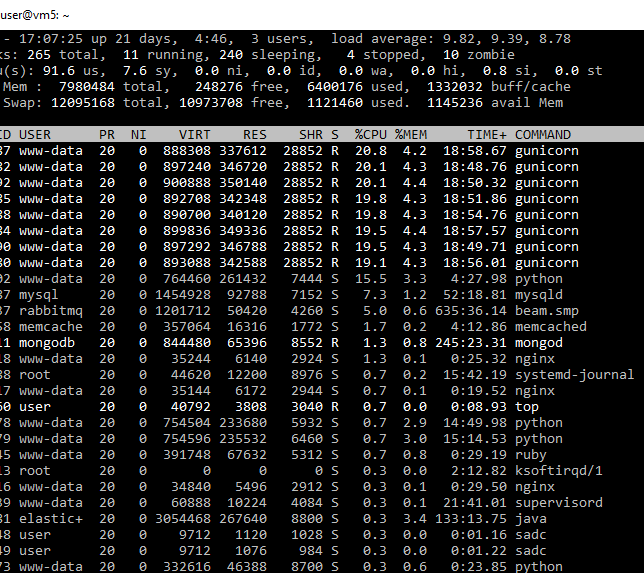
\includegraphics[width=\textwidth,height=\textheight,keepaspectratio]{intro/S2.png}\begin{center}
		\textbf{\Large{Performance Testing Open edX Ironwood Release}}
	\end{center}
	\caption{A look at the top command, 30 minutes into the test. Guincorn, which is a Python Web Server Gateway Interface HTTP Server, takes up most of the CPU resources. }
\end{figure}
\begin{figure}[h!]
	\centering
	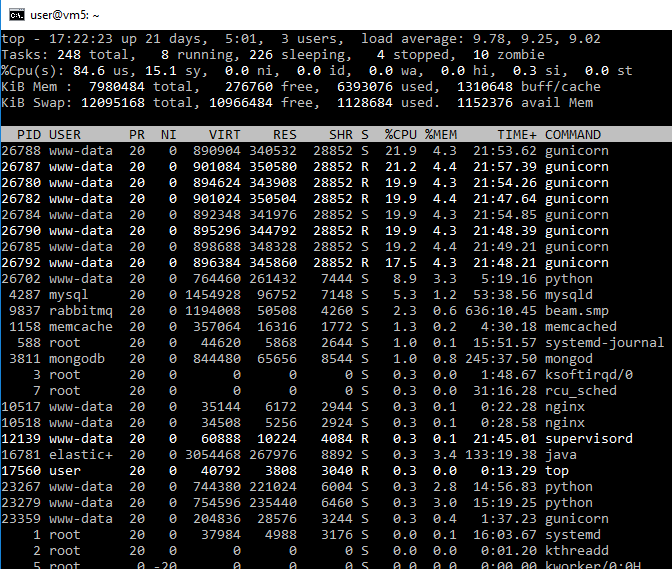
\includegraphics[width=\textwidth,height=\textheight,keepaspectratio]{intro/S3.png}
	\caption{A look at the top command, 45 minutes into the test. Guincorn, which is a Python Web Server Gateway Interface HTTP Server, takes up most of the CPU resources.}
\end{figure}

\begin{figure}[h!]
	\centering
	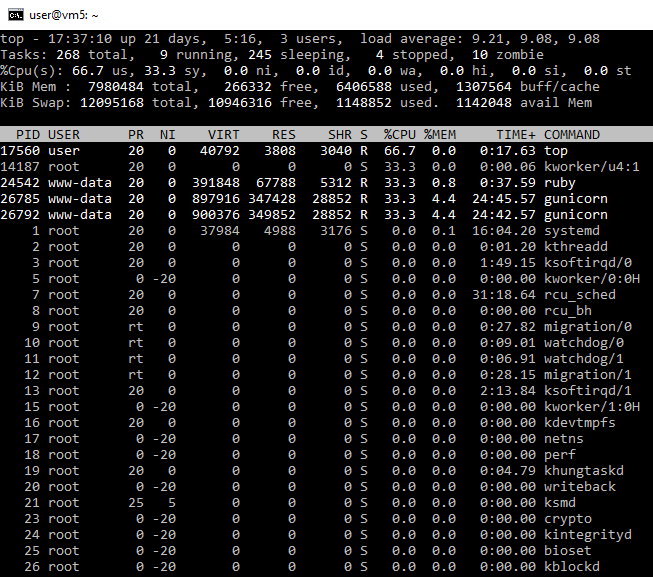
\includegraphics[width=\textwidth,height=\textheight,keepaspectratio]{intro/S4.png}
	\caption{A look at the top command, 60 minutes into the test. Guincorn, which is a Python Web Server Gateway Interface HTTP Server, takes up most of the CPU resources.}
\end{figure}
\clearpage
\section{Testing Open edX Developer Stack (Devstack)}
\subsection{System Configurations}
Here are the details of the hardware and software configuration of the application under test and the client machine that has been used to generate load.
\subsection{Load Generator System Details}
\begin{itemize}
	\item Operating System: Windows 10 Home 64-bit
	\item RAM: 8GB
	\item Processor: Intel(R) Core(TM) i5-7200U CPU @ 2.50GHz x 2 Cores
\end{itemize}
\subsection{Server Configuration}
\begin{itemize}
	\item Operating System: Ubuntu 16.04.4 LTS
	\item RAM: 7.61 GB
	\item Processor: Intel Common KVM Processor @ 2.095 MHz x 2
\end{itemize}
\subsection{Test Details}
\begin{itemize}
	\item Duration: $1$ Hour
	\item Virtual Connections: 10
\end{itemize}
\subsection{Test Results}
The application under test could handle 10 users for the specified server configuration under the current test setup. Furthermore, the test fails for around 15-20 users.
\clearpage
\begin{figure}[h!]
	\centering
	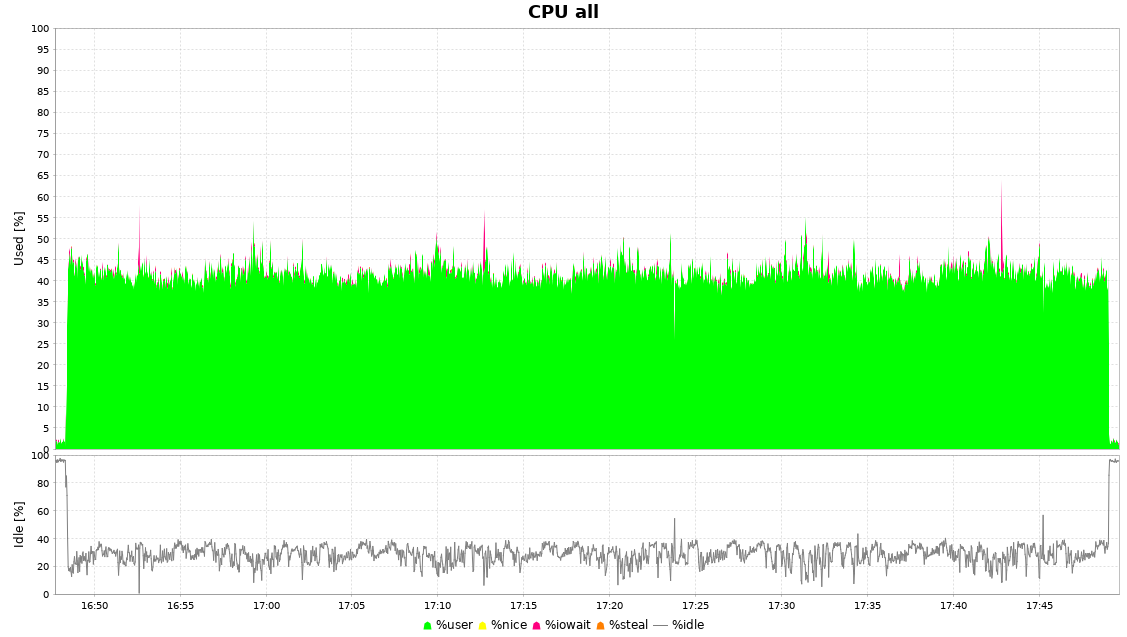
\includegraphics[width=\textwidth,height=\textheight,keepaspectratio]{intro/cpu_harshit.png}
	\caption{SAR CPU Metrics}
\end{figure}
\begin{figure}[h!]
	\centering
	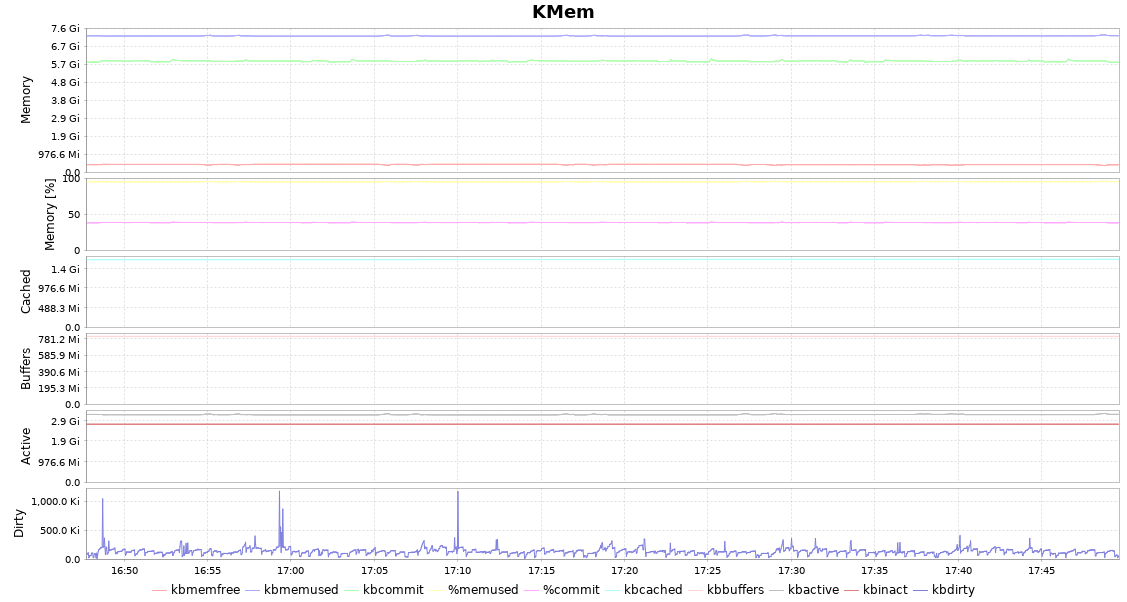
\includegraphics[width=\textwidth,height=\textheight,keepaspectratio]{intro/mem_harshit.png}
	\caption{SAR Memory Metrics}
\end{figure}

\newpage
\begin{figure}[h!]
	\centering
	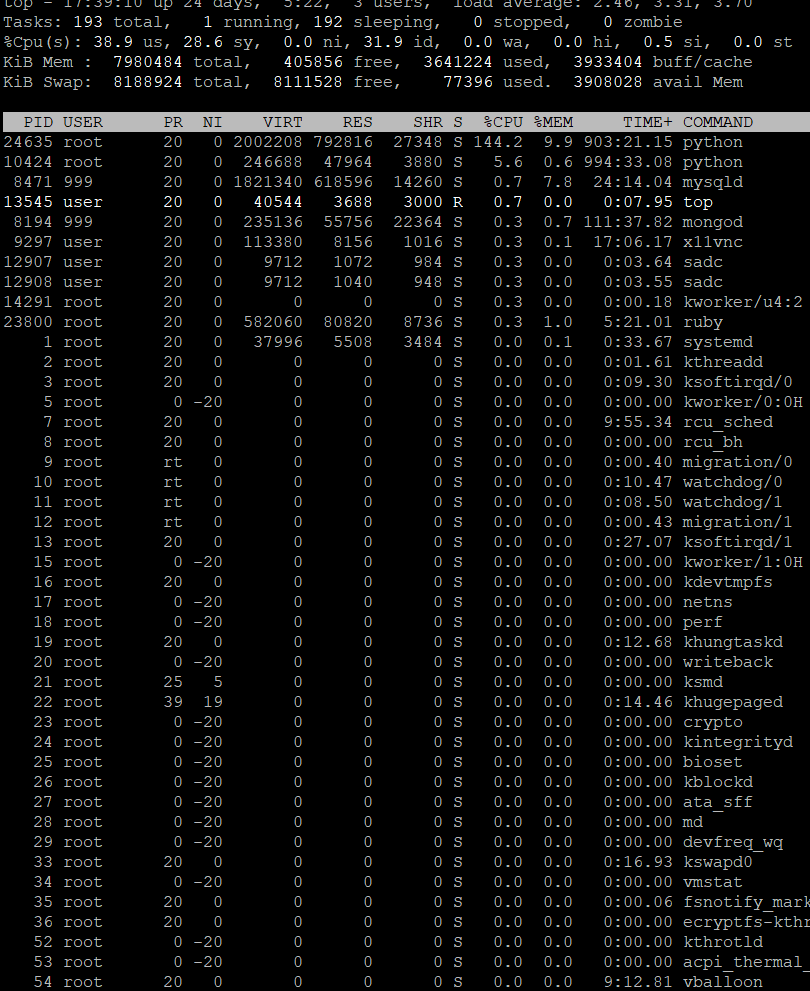
\includegraphics[width=\textwidth,height=\textheight,keepaspectratio]{intro/S1_harshit.png}
	\caption{A look at the top command, 15 minutes into the test. Python takes up most of the CPU Resources.}
\end{figure}
\begin{figure}[h!]
	\centering
	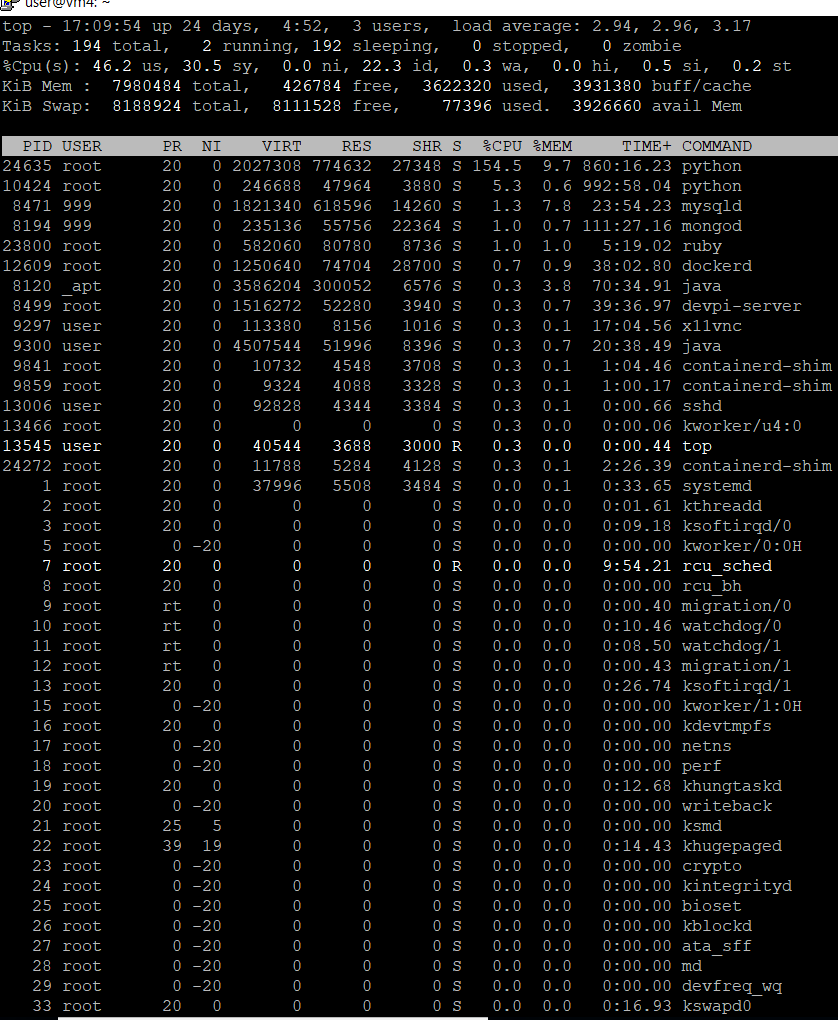
\includegraphics[width=\textwidth,height=\textheight,keepaspectratio]{intro/S2_harshit.png}
	\caption{A look at the top command, 30 minutes into the test. Python takes up most of the CPU Resources.}
\end{figure}

\begin{figure}[h!]
	\centering
	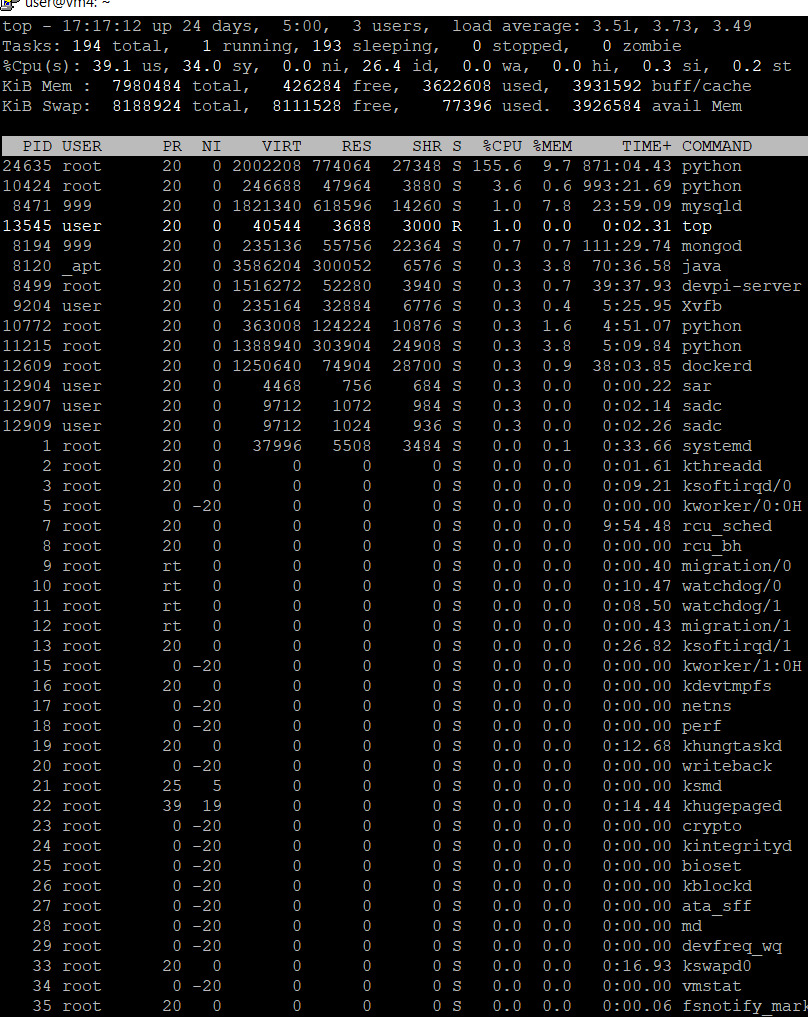
\includegraphics[width=\textwidth,height=\textheight,keepaspectratio]{intro/S3_harshit.png}
	\caption{A look at the top command, 45 minutes into the test. Python takes up most of the CPU Resources.}
\end{figure}

\begin{figure}[h!]
	\centering
	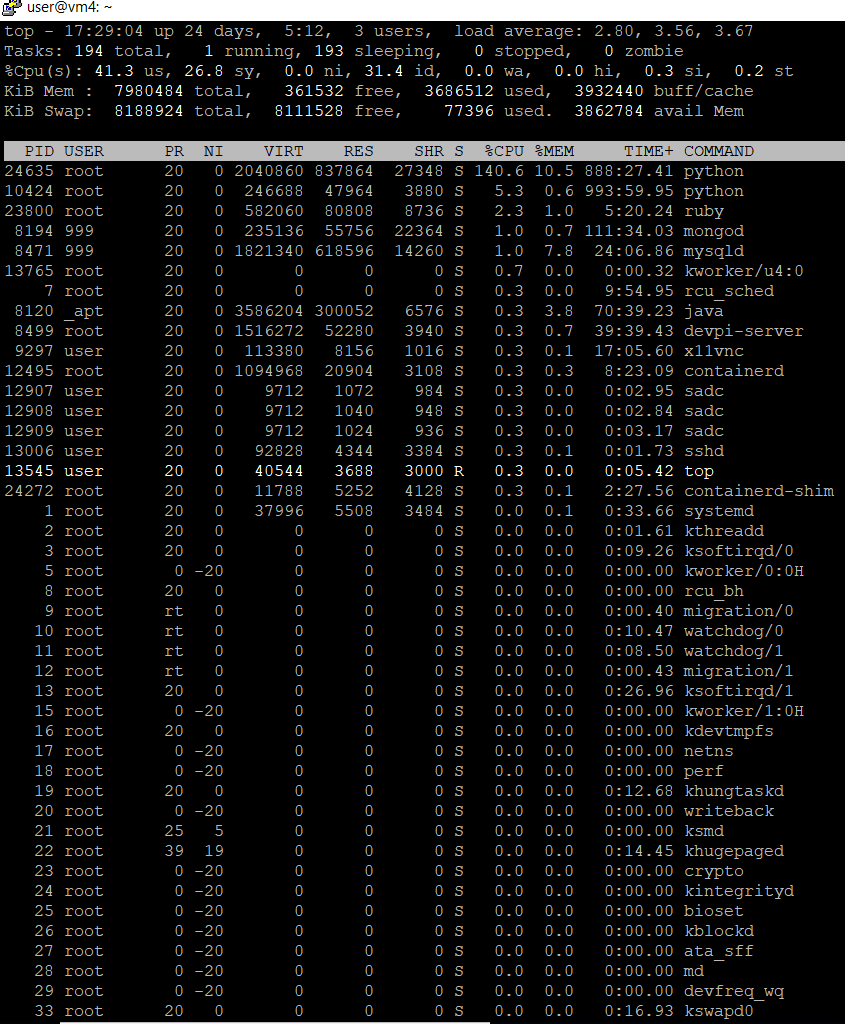
\includegraphics[width=\textwidth,height=\textheight,keepaspectratio]{intro/S4_harshit.png}
	\caption{A look at the top command, 60 minutes into the test. Python takes up most of the CPU Resources.}
\end{figure}

\begin{figure}[h!]
	\centering
	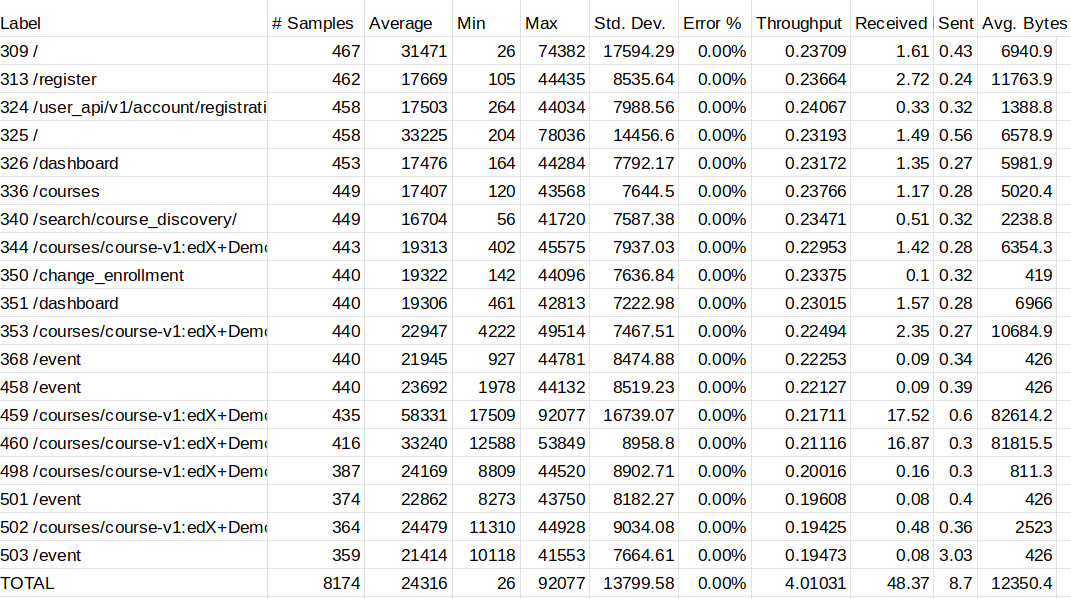
\includegraphics[width=\textwidth,height=\textheight,keepaspectratio]{intro/3.png}
	\caption{JMeter Summary Report for Open edX Native.}
\end{figure}

\begin{figure}[h!]
	\centering
	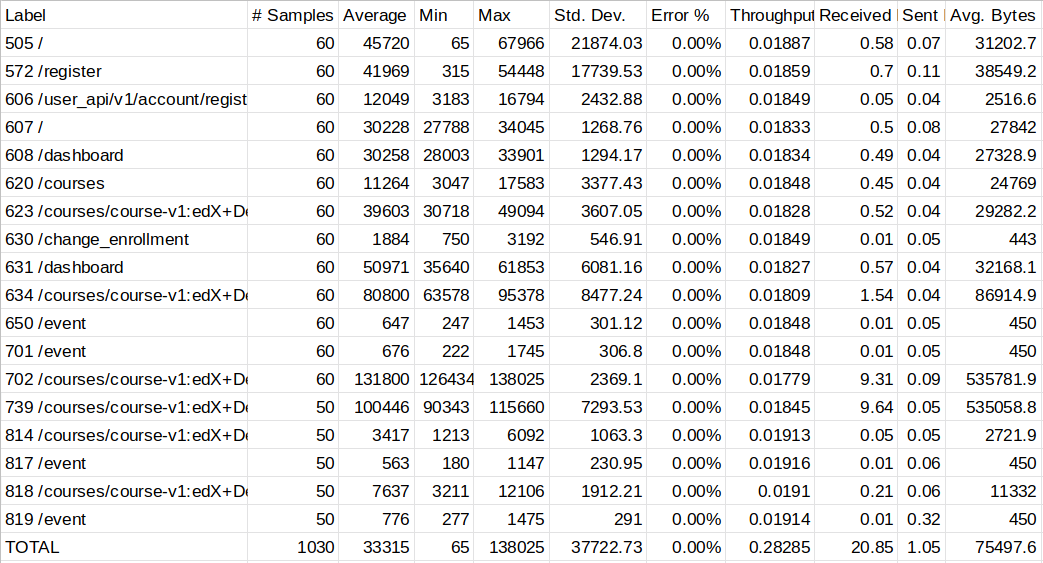
\includegraphics[width=\textwidth,height=\textheight,keepaspectratio]{intro/4.png}
	\caption{JMeter Summary Report for Open edX Devstack.}
\end{figure}
\clearpage
\section{Test Results} 
\begin{itemize}
	\item Under the current test setup and server configurations, it is evident that Open edX Native can handle around $100$ virtual connections, which is much better than $10$, the number of virtual connections that could be handled by Open edX Devstack.
	\item In $1$ hour, the total number of transation completed by Open edX Native was $8174$, much more than that of Open edX Devstack, which amounted to $1030$.
	\item Furthermore, the average response time of Open edX Native is $24.316$ seconds, which outperforms Open edX Devstack, whose average response time is $33.313$ seconds.
	\item Along with that, the throughput, which has been measured in requests/sec, for Open edX Native is $4.01$, whereas it is $0.28$ for Open edX Devstack.
	\item As for the CPU Utilization, Open edX Native consumes around 85-95\% of CPU Resources, which is much more than the CPU Utilization of Open edX Devstack (40-50\%).
	\item The memory consumption was close to 100\% in both the setups.
	\item A closer look at the Summary Reports shows that the response time recorded corresponding to the case where the enrolled course's dashboard is accessed is very high, relative to other requests in a given test plan. Moreover, this response time is exceedingly high for Open edX Devstack.
\end{itemize}

\par
The official Open edX documentation states that nginx and gunicorn have been disabled in Devstack. Hence, it uses Django's runserver as an alternative. This can be verified by the top command's result as shown in figures 14-17, 20-23.


\bibliographystyle{ieeetr}
\bibliography{biblio}


\end{document}